\section{Background and Motivation}
\label{sec:motivation}

\para{Background:} 


\begin{figure*}[h]  
	\centering   
	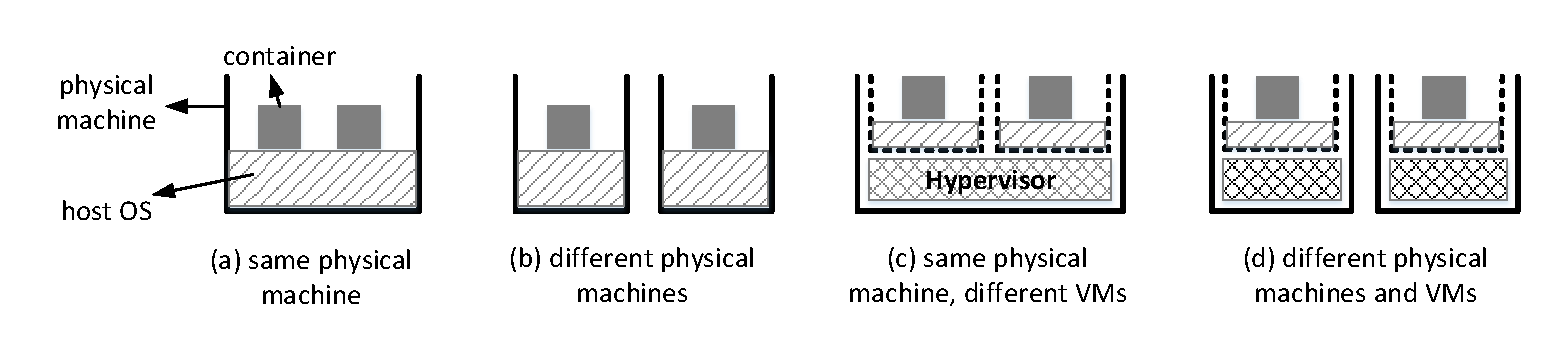
\includegraphics[width=6.7in]{figures/deployment-cases}   
	\caption{\label{fig:deploy-cases} Representative running environments of containers.}   
\end{figure*}

Most containerized applications are usually composed of multiple containers. For
example, each master and slave node in Hadoop is an individual container; A web
service can include layers, such as load balancer, web server, in-memory cache
and backend database, and each layer can be a distributed system with multiple
containerized nodes. These containers are usually deployed into a multi-host
server cluster, and the deployment is usually controlled by a cluster
orchestrator, e.g. Mesos~\cite{xxx}.  Such architecture makes it easier to
upgrade the nodes or mitigate failures, since a stopped container can be quickly
replaced by a new one on the same or a different host.  Working as a single
application, containers need to exchange data, and the network performance has a
significant impact on the overall application performance~\cite{coflow-etc.}

Depending on whether containers run on bare-metal hosts or VM hosts,
Figure~\ref{fig:deploy-cases} illustrates the four cases any container
networking solution must handle. For maximum portability, containers today often
use ovelay networks as shown in Figure~\ref{fig:overlay}. A number of software
solutions are available to provide this overlay fabric, including
Weave~\cite{wave} and Calico~\cite{calico}. The host (i.e. the server or the VM)
runs software router. The router connect to the NIC of the host. It also
connects with the virtual interfaces of the containers on the host via a
software bridge. It performs appropriate tunneling (encapsulation and
decapsulation) to move traffic between the physical network and the overlay
fabric. The router uses standard networking protocols like BGP to connect with
software routers on other hosts. Containers send and receive IP packets via this
overlay, and hence are agnostic to location of other containers they are
communicating with.

The CPU overhead of processing packets in the software bridge, as well as in the
software router (for off-host communication) is the primary bottleneck to the
performance of this overlay.

%% In this paper, we focus on the cases (a) and (b) in
%% Figure~\ref{fig:deploy-cases} and discuss how to support the other two cases in
%% the future.

\subsection{Existing container overlay networks}

\vyas{seems like a logical disconnect to me .. why is there a section on overlay networks?}

\vyas{i would keep it simple as follows: 2.1 -- background 2.2 -- measurements 2.3 -- insights. dont get too fancy 
 in subsection titles/structure}

\begin{figure}[h]  
	\centering   
	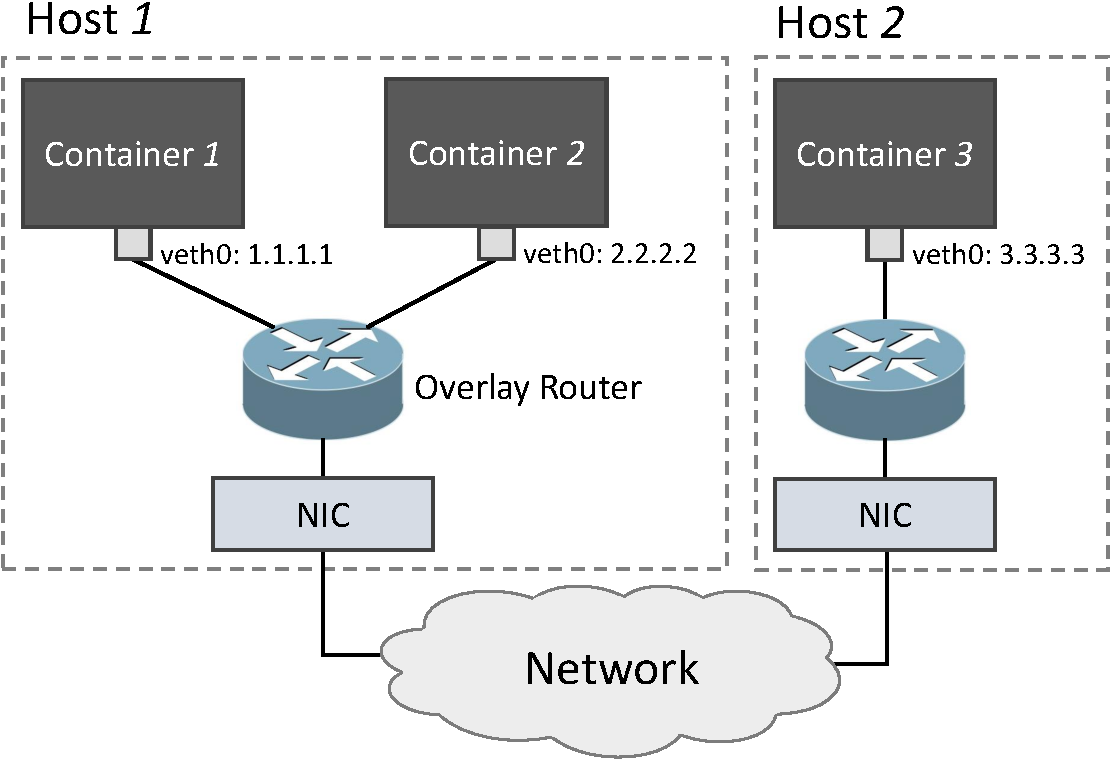
\includegraphics[width=0.8\linewidth]{figures/overlay.pdf}   
	\caption{\label{fig:overlay} The design of existing container overlay networks (Weave).}   
\end{figure}   


\subsection{Opportunities for better networking}

The key to achieve a high performance and low overhead overlay network
for containers is bypassing the performance bottlenecks, including
bridges, software routers and host OS kernel, on data-plane. Given that
containers are essentially processes, the communication channels provided
by IPC and hardware offloading techniques give us numerous hammers to 
build a better container network. For instance, 
containers within a single host (like Container-1 and 
Container-2 in Figure~\ref{fig:overlay}) can communicate via 
shared-memory and software routers in different hosts can talk via RDMA, 
which helps to bypass performance bottlenecks.

To understand the network performance and overhead when containers
talk via shared-memory and RDMA \footnote{In this paper, we choose RDMA
as a representative hardware offloading technique, and we will consider other
alternatives in the future.}, we conducted network bandwidth and latency benchmarks between two containers. In the shared-memory case, the sender
container opens a pieces of shared memory and write data into it, and 
the receiver container can read the memory once it gets the pointer of 
the shared memory from the sender; In the RDMA case, both the sender
and the receiver use host modes and communicate with the standard RDMA API
over the host NICs. We use Weave to in the evaluation of existing overlay
networks. The results are shown in Figure XXX.

     \begin{figure}[ht]
     \centering 
     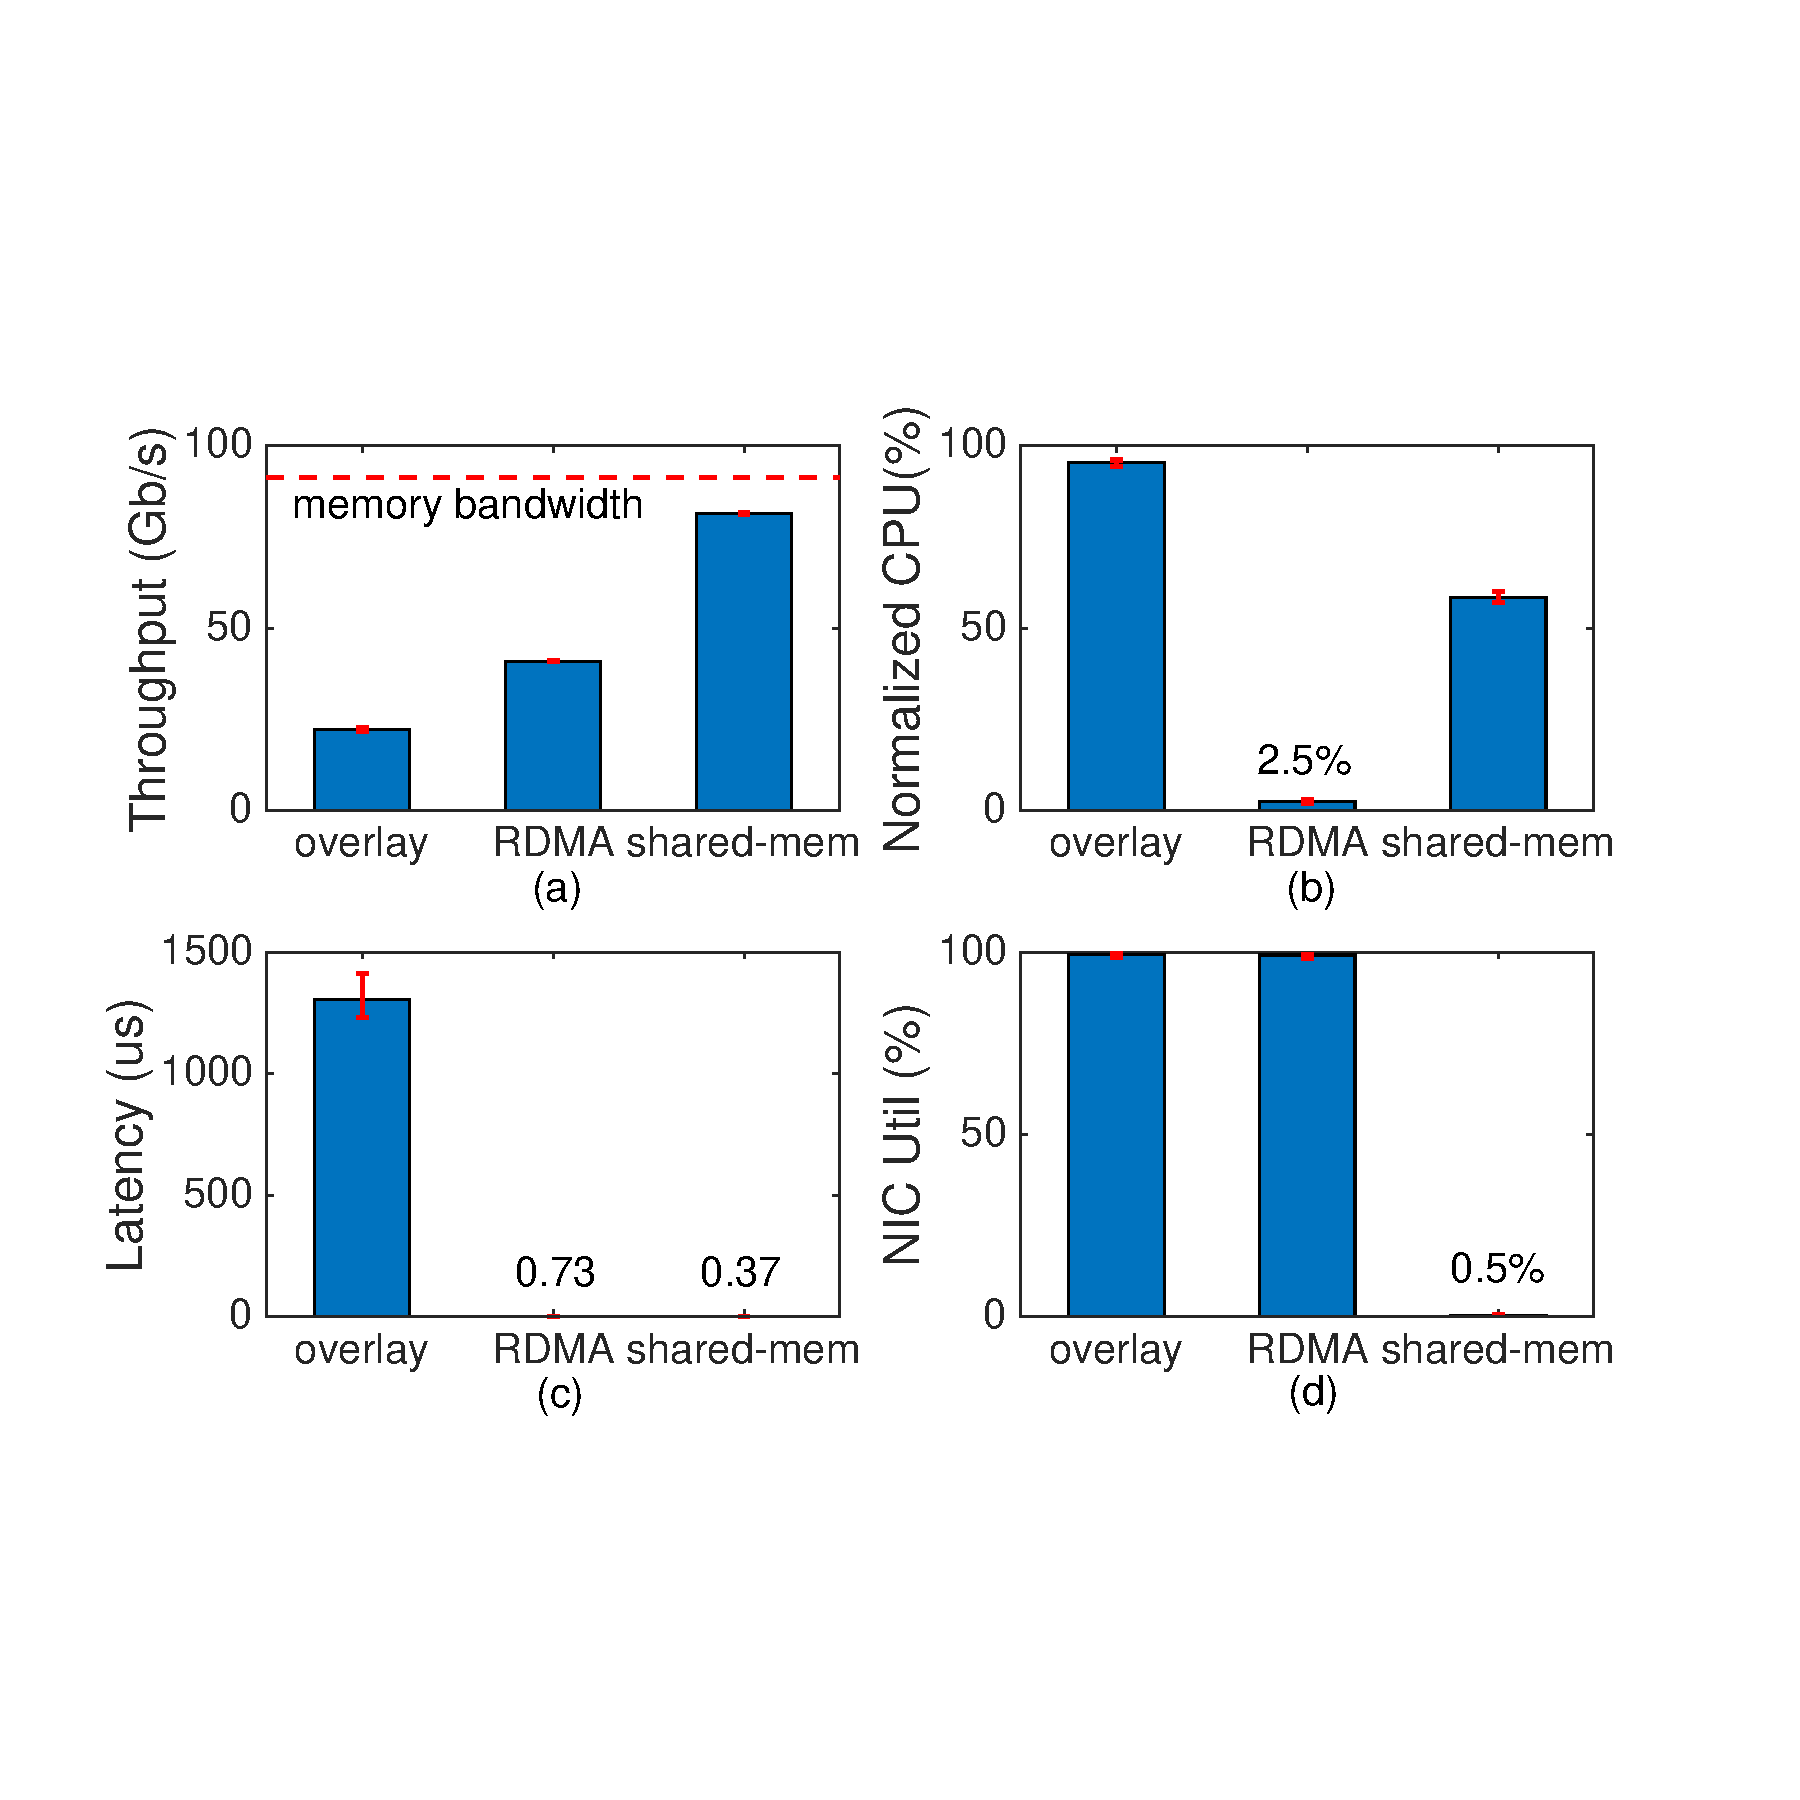
\includegraphics[width=0.5\textwidth]{figures/motivation/mot_rdma_shm.pdf}      
     \label{fig:mot_rdma_shm}
     \caption{The throughput, CPU usage, latency and NIC utilization for a pair of 
     containers communicating via overlay network, RDMA or shared memory.} 
     \end{figure}

Figure~\ref{fig:eval_baremetal_thr} shows that in intra-host cases, the bandwidth between two
containers can reach the NIC speed at about 40Gbps then RDMA is used and 
even exceed the limitation of NIC speed to approach to memory bandwidth when
they use shared-memory is used. As shown in Figure The price of the high bandwidth of shared-memory is high CPU utilization due to data-copying when the sender writes data into
the shared-memory, while RDMA has negligible CPU overhead because it directly uses NICs and DMA controllers for data copying and packet processing.
Figure~\ref{fig:eval_exist_latency} show the latency when a sender 
transfers XXX bytes to the receiver. We can see that both shared-memory
and RDMA have XXX orders of magnitudes reduction in latency compared with Weave.
Overall, we can conclude that both shared-memory and RDMA have 
significant improvement in network performance and reduction in CPU overhead,
compared with existing overlay networking solutions.

     \begin{figure}[ht]
     \centering 
     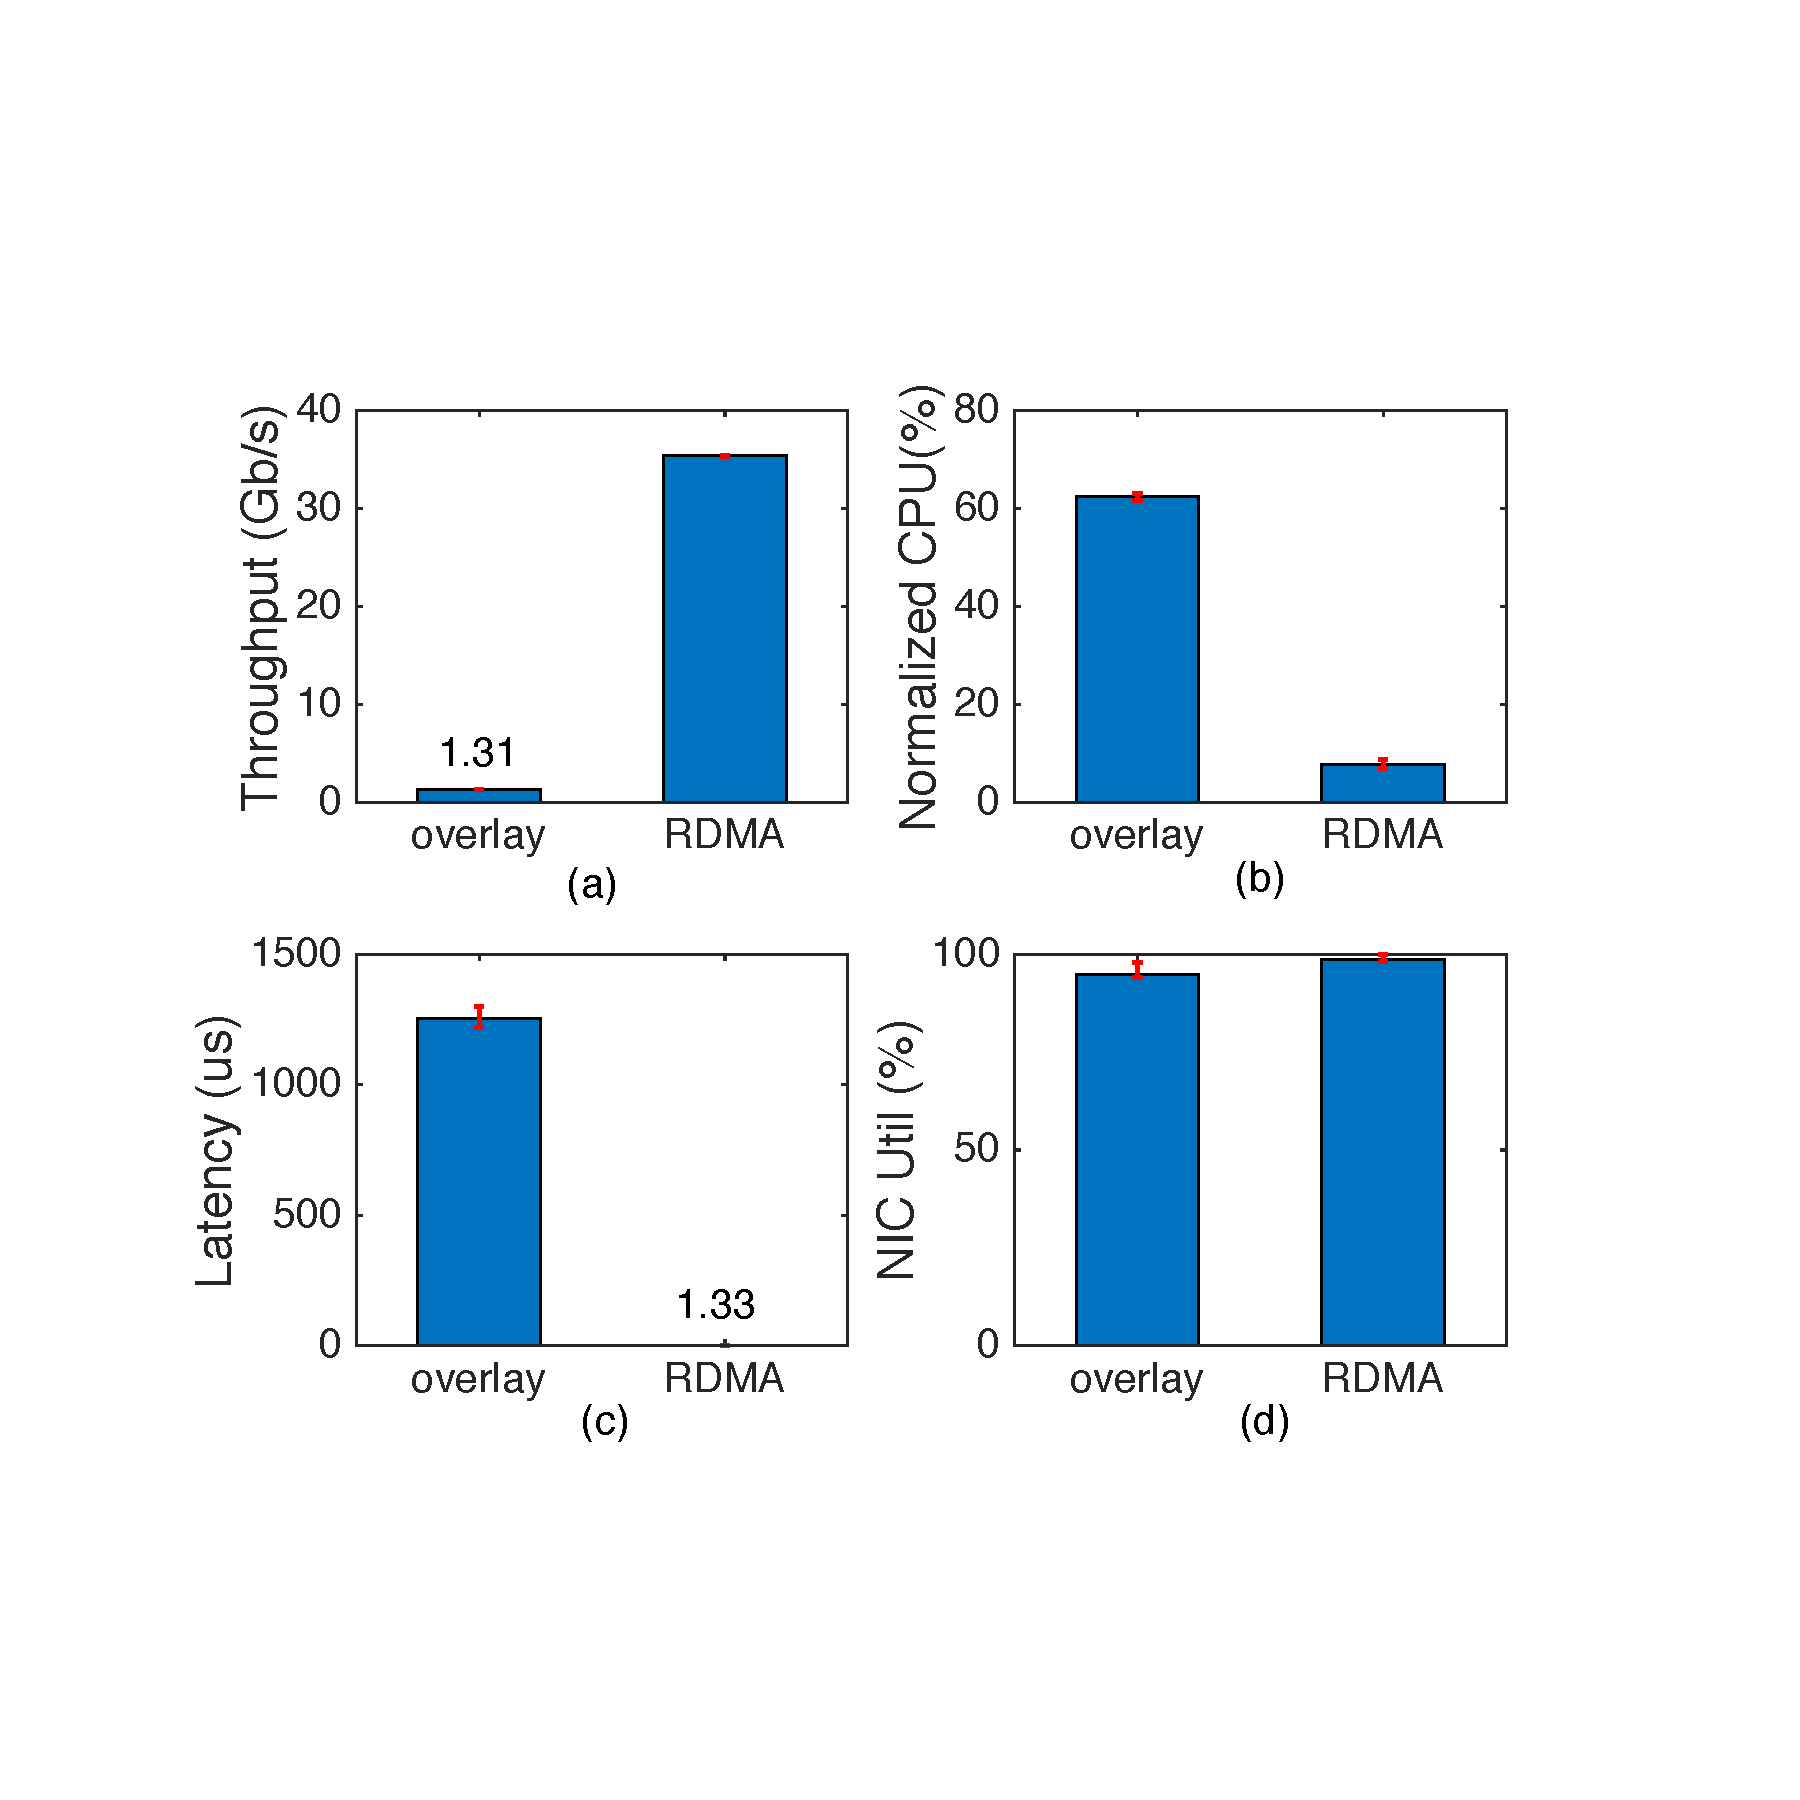
\includegraphics[width=0.5\textwidth]{figures/motivation/mot_rdma_inter.pdf}      
     \label{fig:mot_rdma_inter}
     \caption{The throughput, CPU usage, latency and NIC utilization for a pair of 
     containers communicating via overlay network, RDMA or shared memory in 
     inter-host setting.} 
     \end{figure}
     
 \tianlong{Here we need a paragraph say for inter-host setting, we can use RDMA to achieve high bw, low latency.}

Therefore, we have a huge opportunity to achieve a high performance
and low overhead network if we can enable shared-memory and RDMA 
in the data-plane of container overlay networks.

\subsection{Challenges}

(1) Using standard APIs, transparent to containers;


(2) Smoothly integrating shared-memory and RDMA according to containers' locations.

(3) Optimizations like removing unnecessary data copies.

%%% commented content 
\iffalse

%Throughput:
     \begin{figure}[ht]
     \centering 
     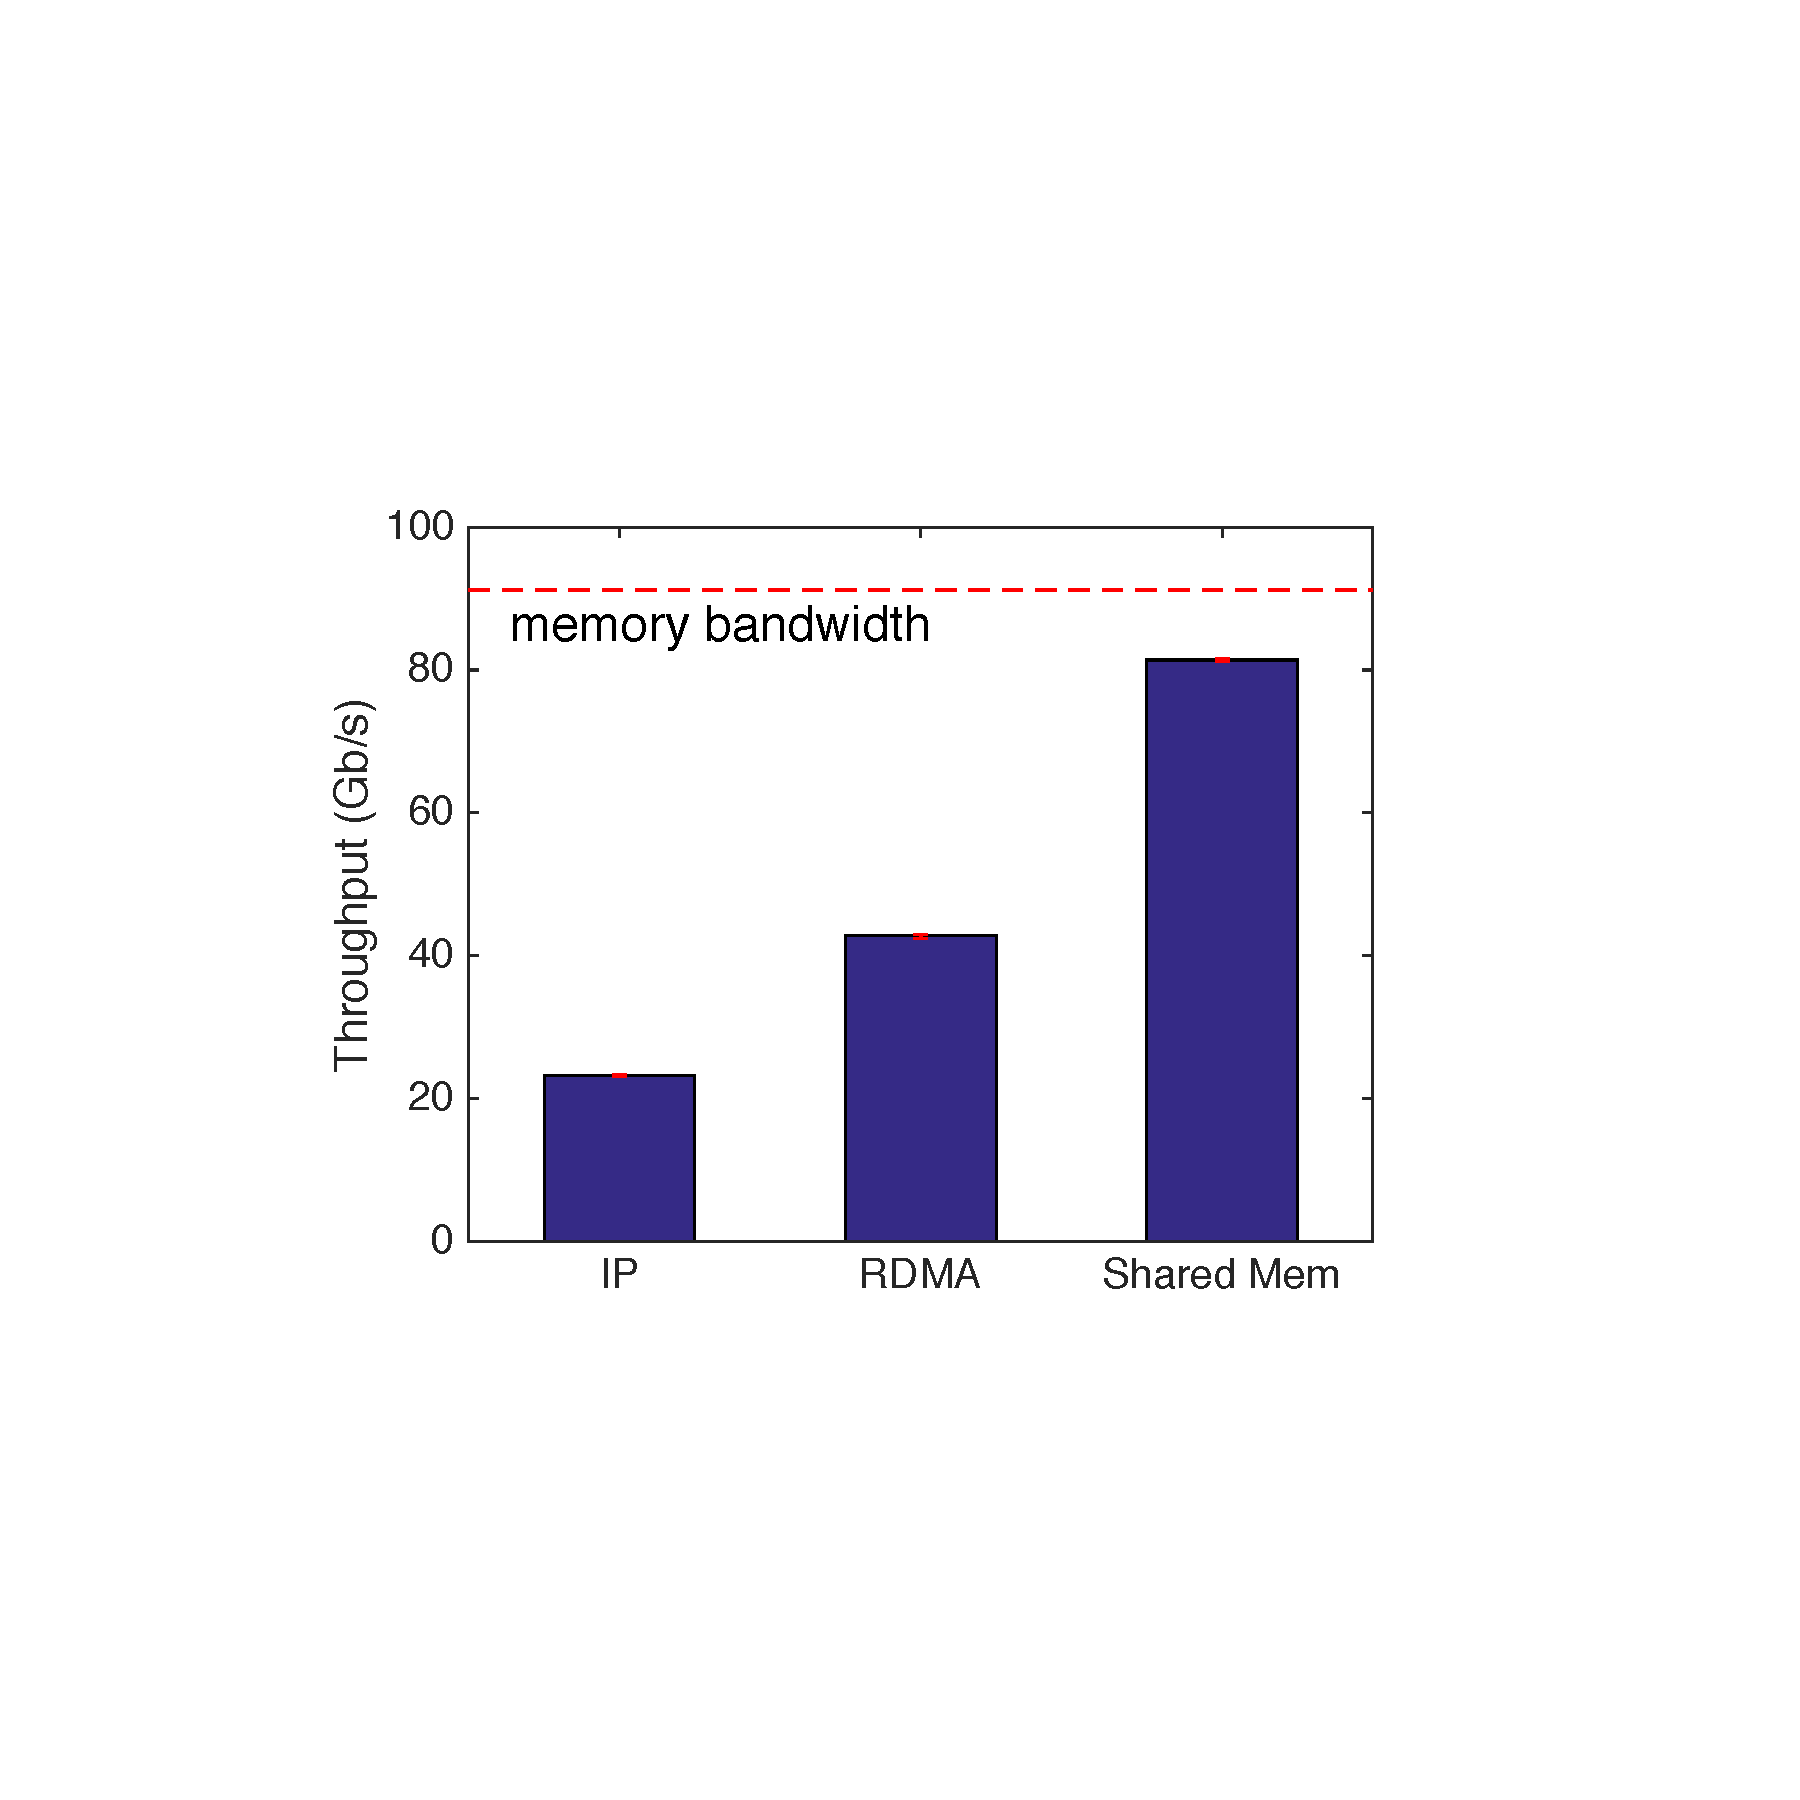
\includegraphics[width=0.32\textwidth]{figures/motivation/eval_baremetal_thr.pdf}      
     \label{fig:eval_baremetal_thr}
     \caption{} 
     \end{figure}

%Latency:    
     \begin{figure}[ht]
     \centering 
     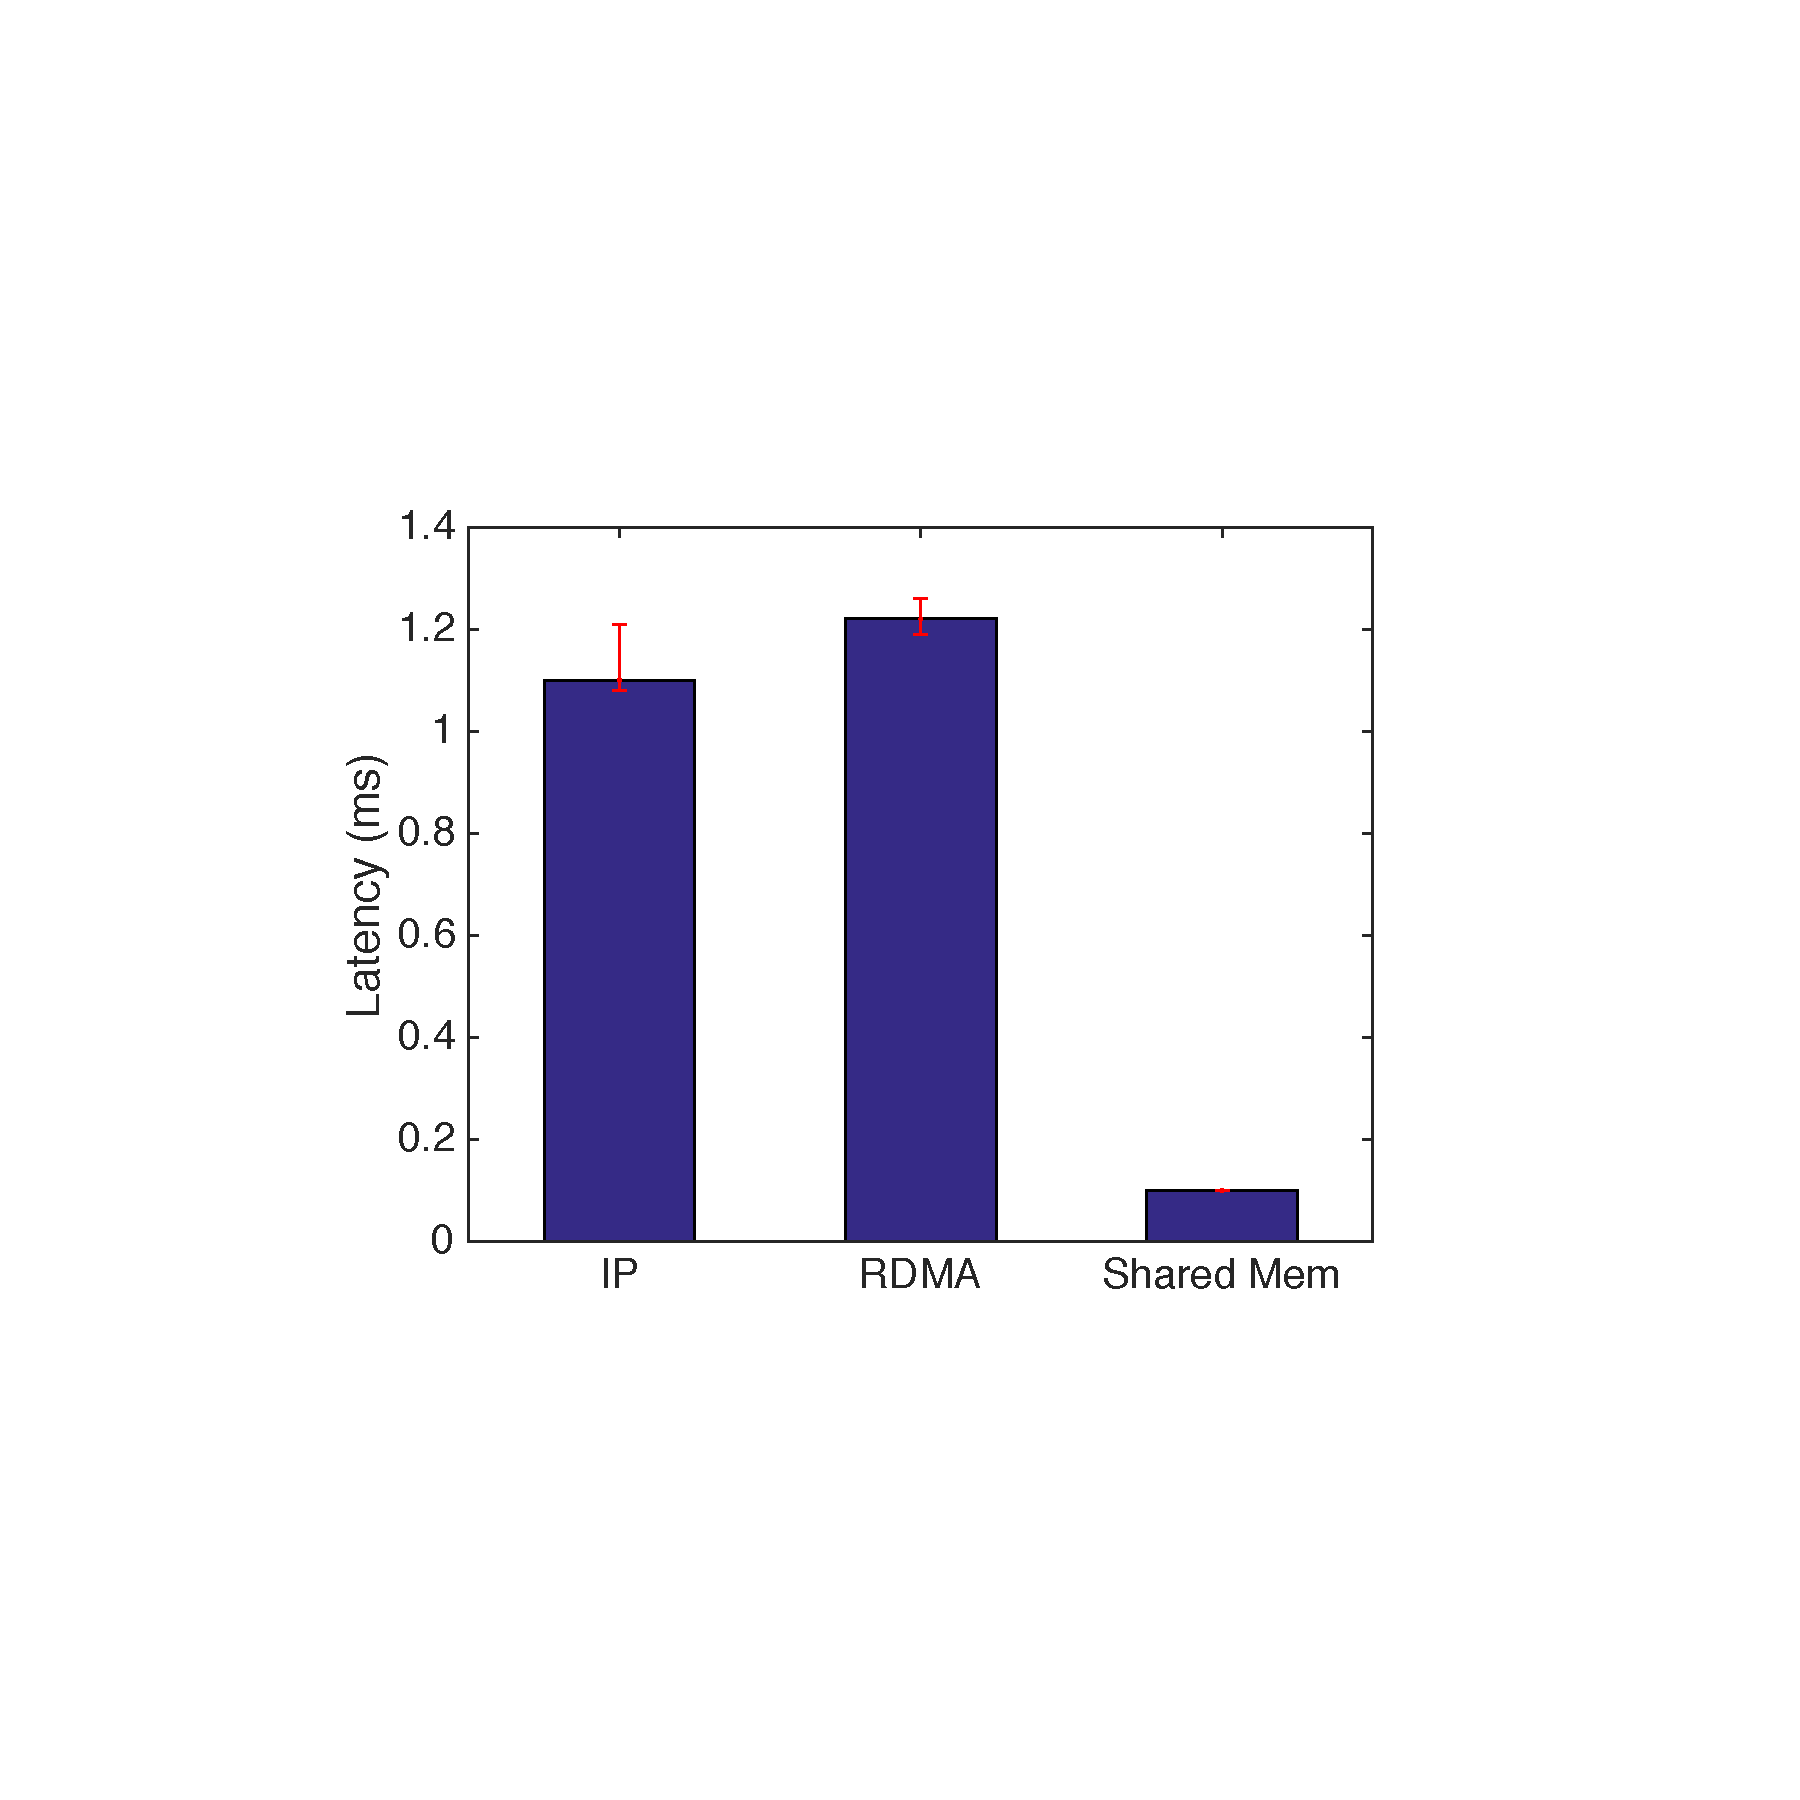
\includegraphics[width=0.32\textwidth]{figures/motivation/eval_baremetal_latency.pdf}      
     \label{fig:eval_baremetal_latency}
     \caption{} 
     \end{figure}

%CPU usage:     
     \begin{figure}[ht]
     \centering 
     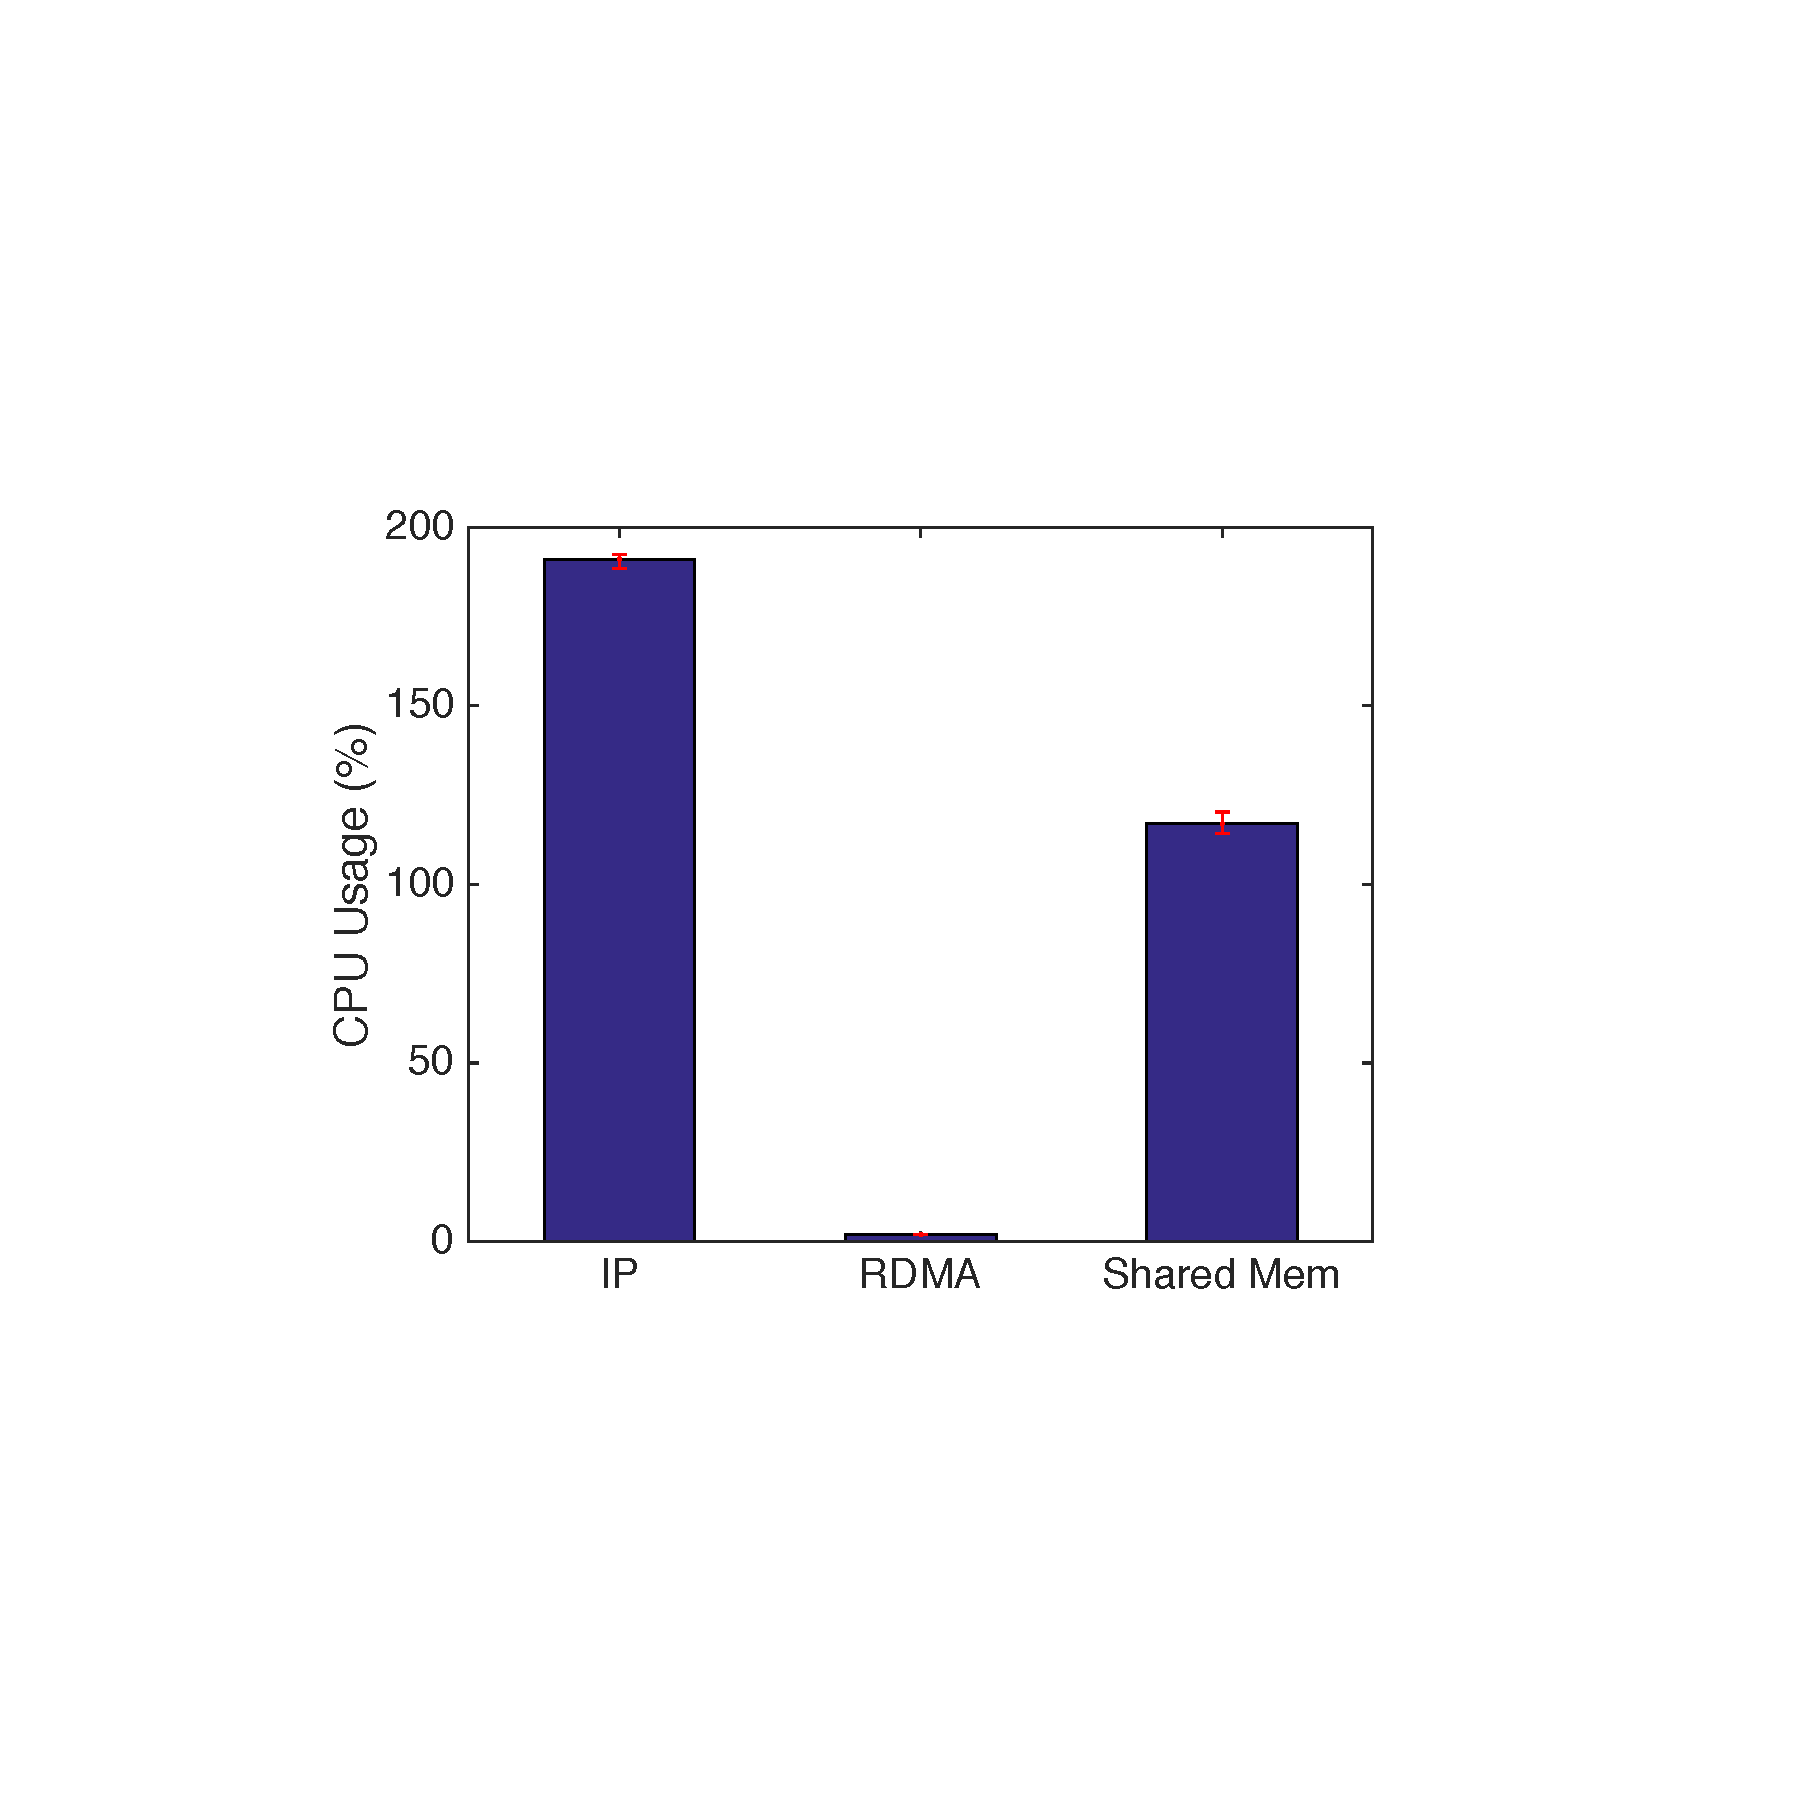
\includegraphics[width=0.32\textwidth]{figures/motivation/eval_baremetal_cpu.pdf}      
     \label{fig:eval_baremetal_cpu}
     \caption{} 
     \end{figure}

\begin{figure}[ht]
     \centering 
     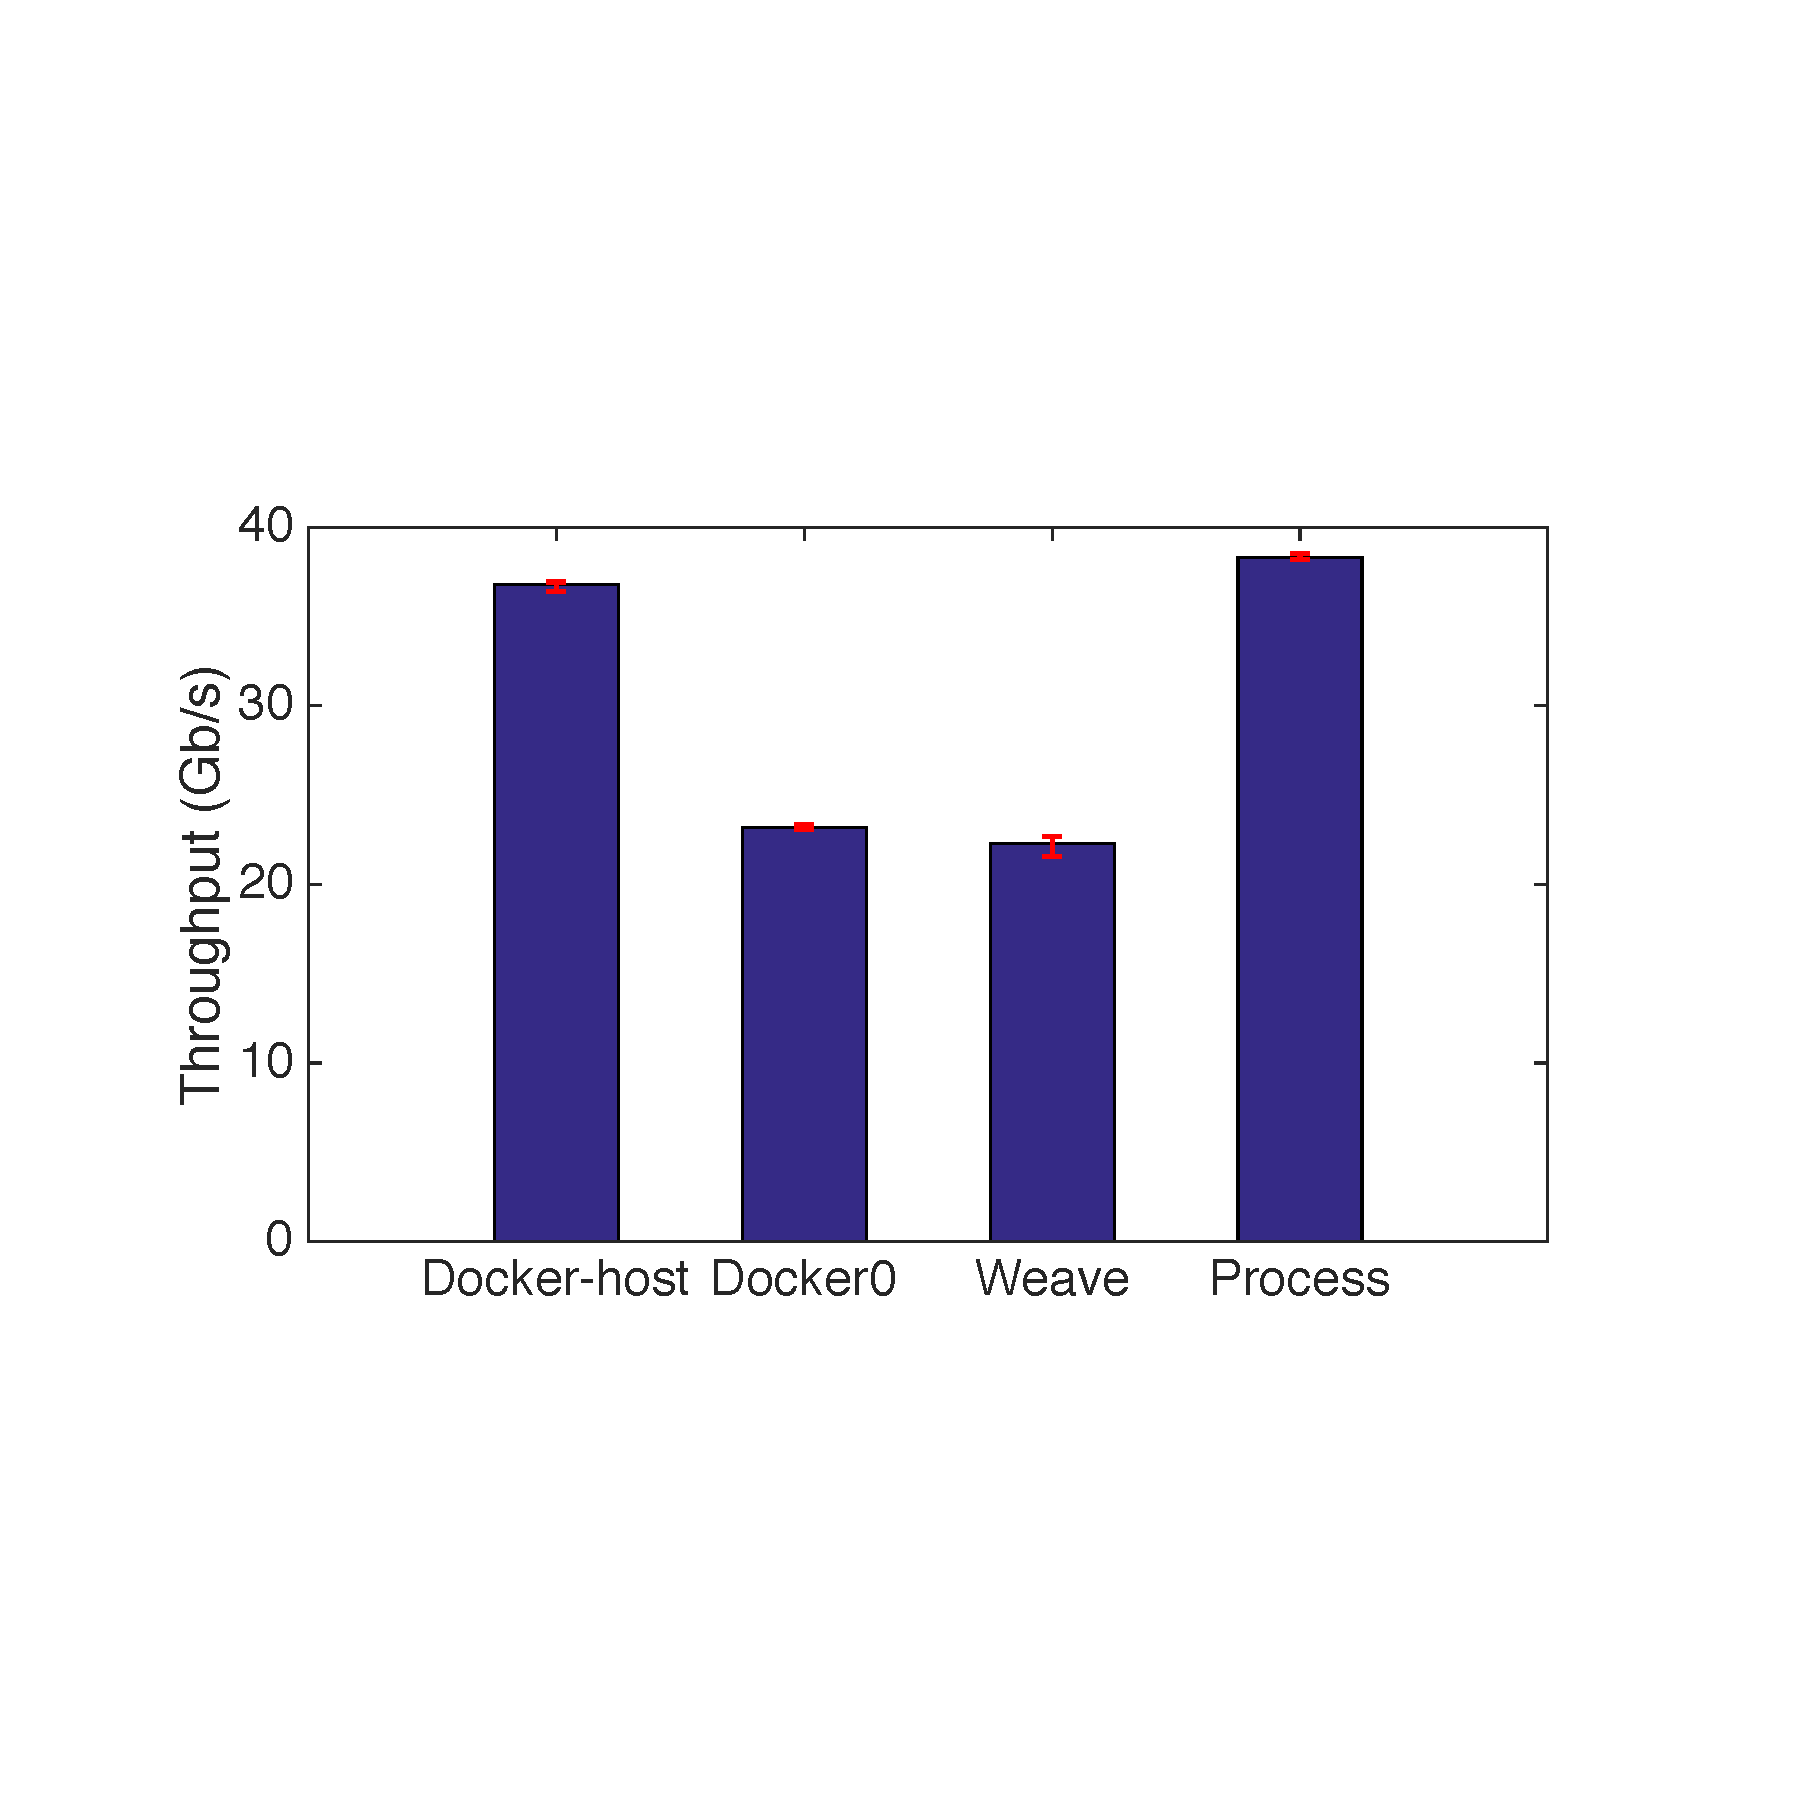
\includegraphics[width=0.4\textwidth]{figures/motivation/eval_exist_bw.pdf} 
     \label{fig:eval_exist_bw}
     \caption{The intra-host throughput of existing solutions. Docker-host is in host mode; Docker0 is in bridge mode; Weave is in overlay mode.} 
\end{figure} 

\begin{figure}[ht]
     \centering 
     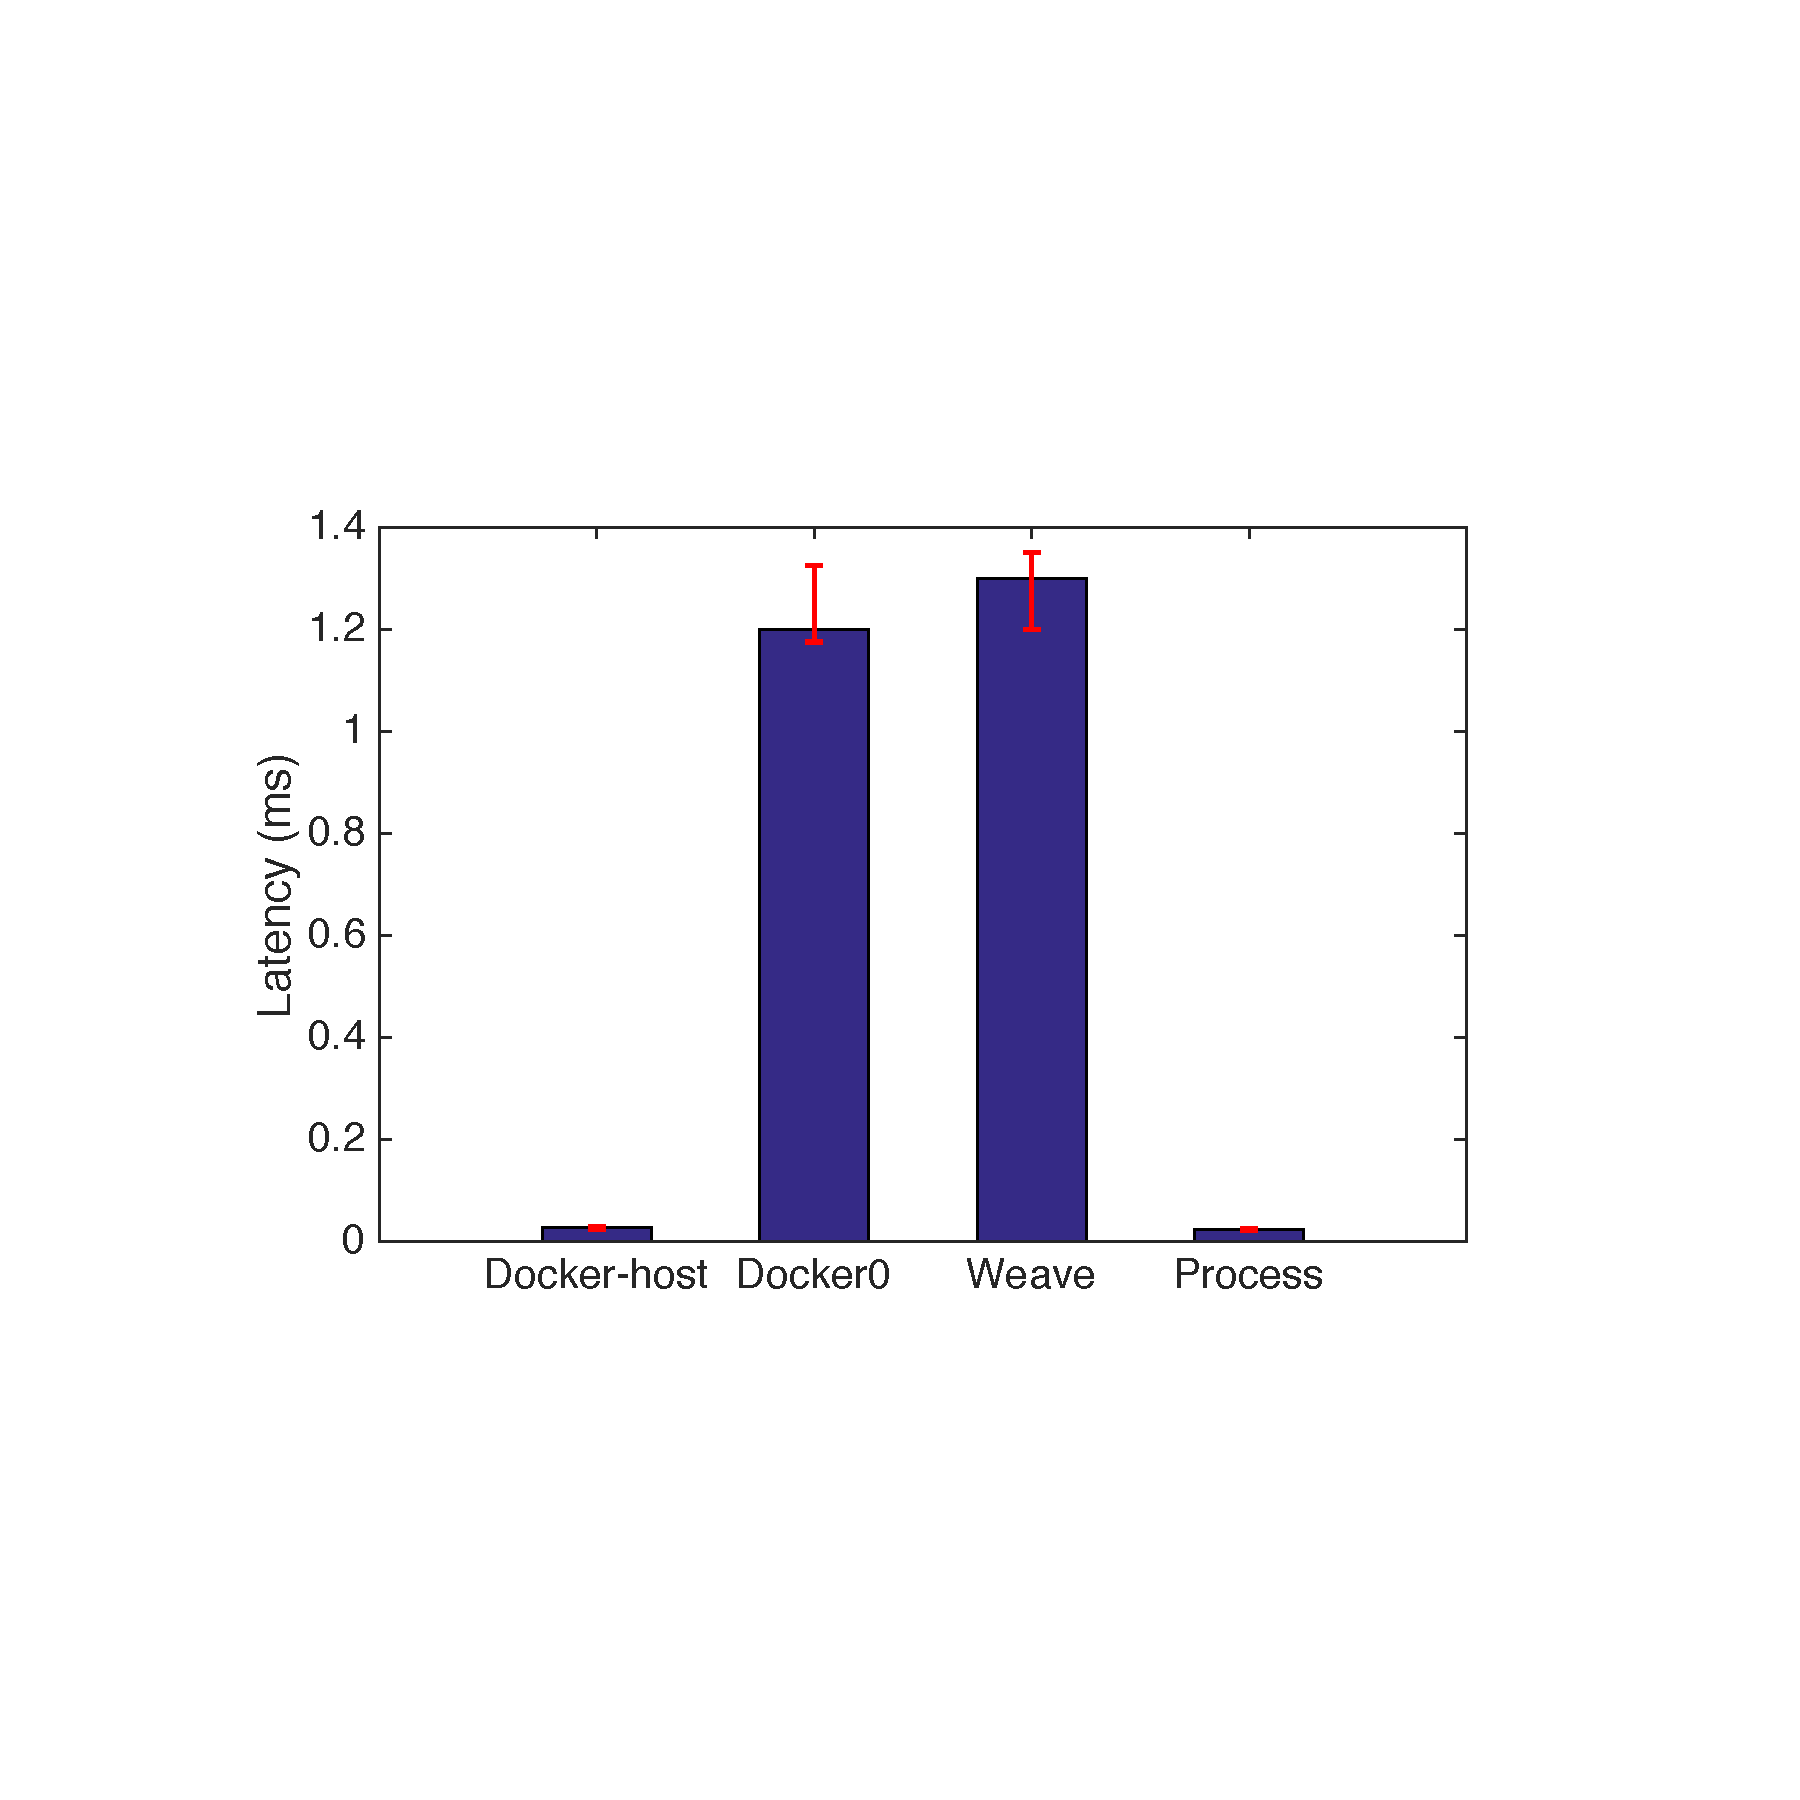
\includegraphics[width=0.4\textwidth]{figures/motivation/eval_exist_latency.pdf} 
     \label{fig:eval_exist_latency}
     \caption{The intra-host latency of existing solutions. Docker-host is in host mode; Docker0 is in bridge mode; Weave is in overlay mode.} 
\end{figure} 

\begin{figure}[ht]
     \centering 
     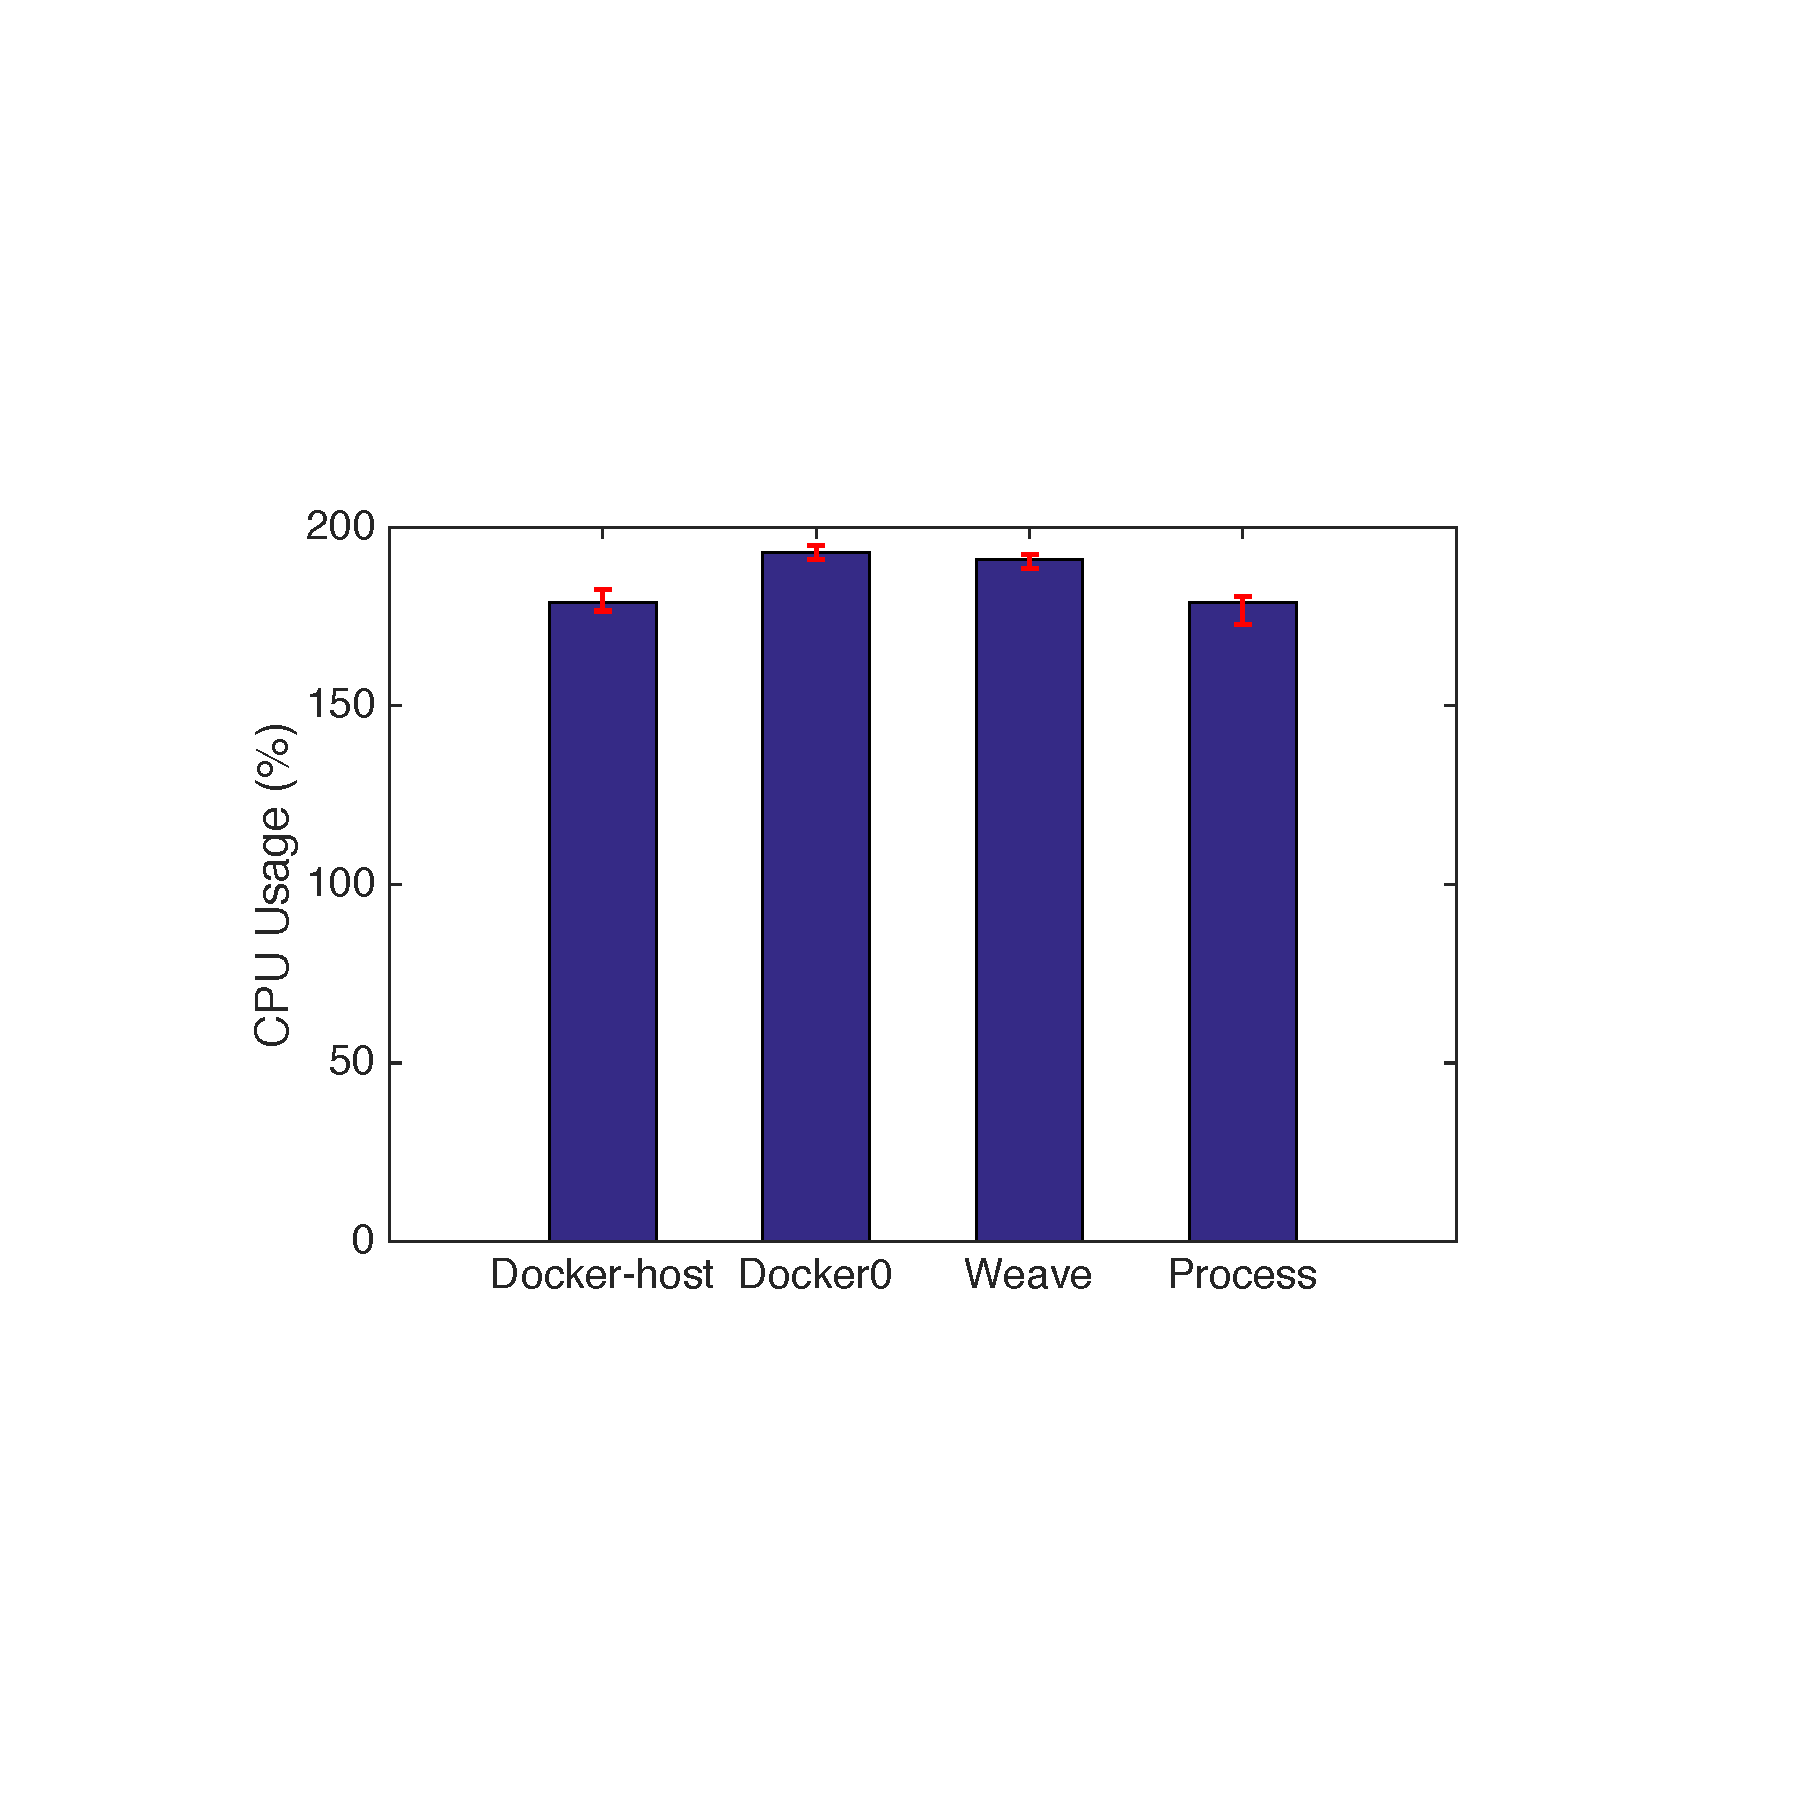
\includegraphics[width=0.4\textwidth]{figures/motivation/eval_exist_cpu.pdf} 
     \label{fig:eval_exist_cpu}
     \caption{The cpu usage of existing solutions. Docker-host is in host mode; Docker0 is in bridge mode; Weave is in overlay mode.} 
\end{figure} 

\begin{figure}[ht]
     \centering 
     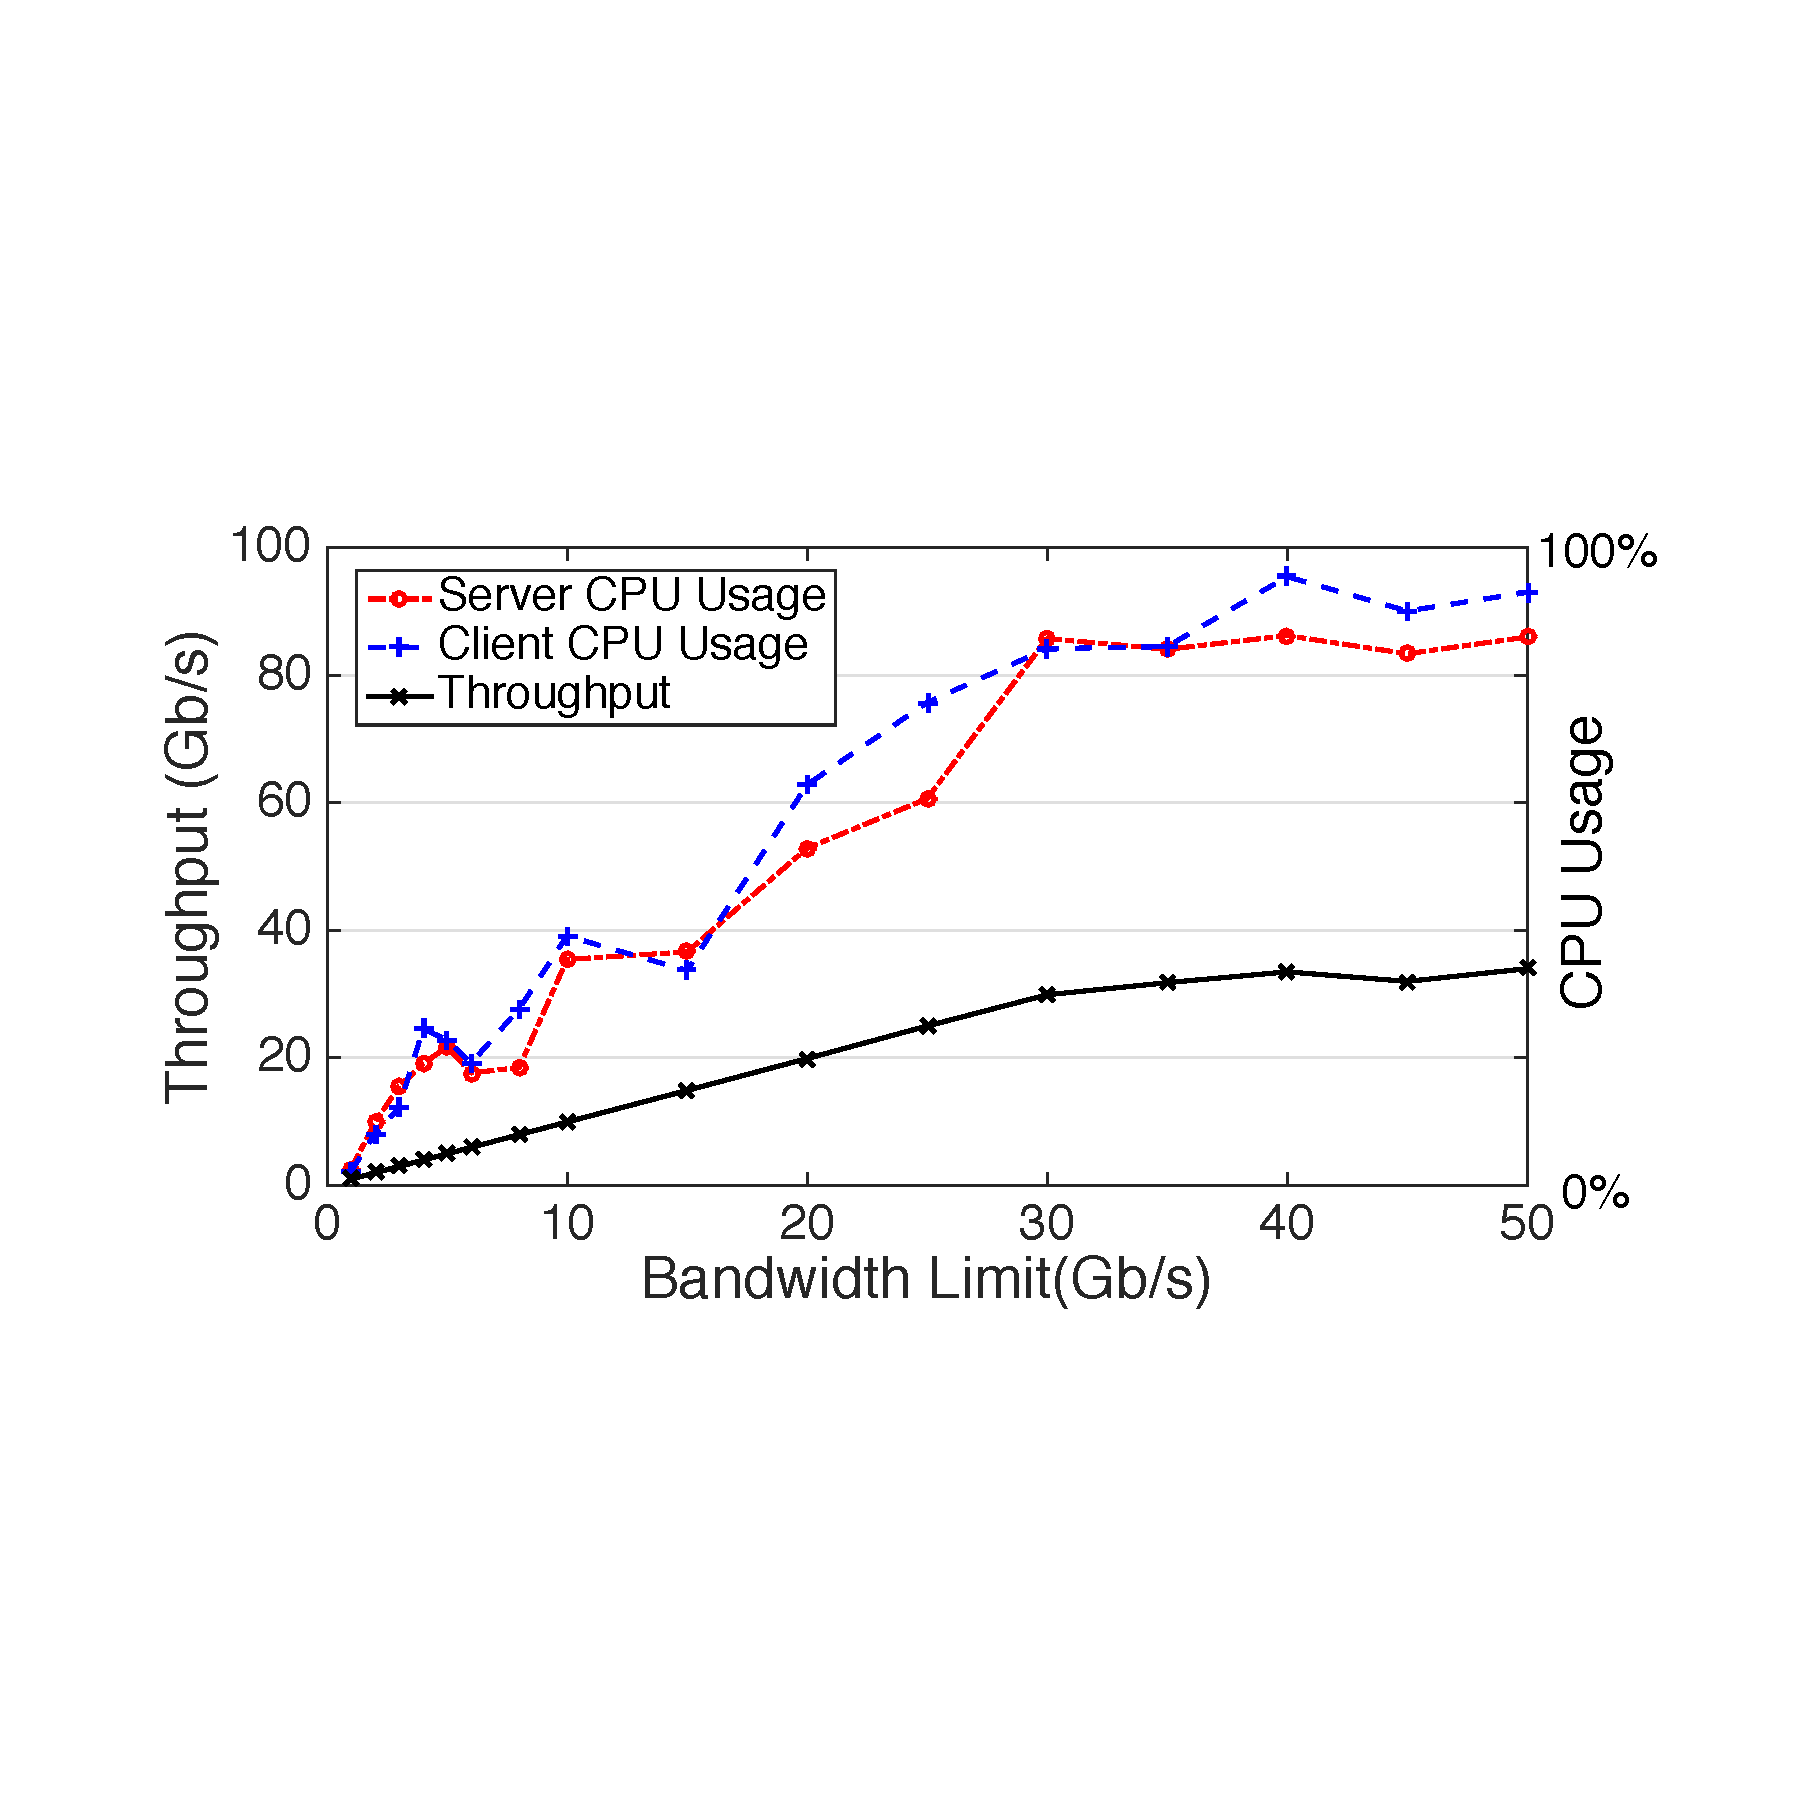
\includegraphics[width=0.4\textwidth]{figures/motivation/eval_bw_cpu.pdf}      
     \label{fig:eval_bw_cpu}
     \caption{} 
\end{figure}


* Figures:

* Throughput comparison (intra- and inter-host)

* CPU comparison

* Latency comparison

In this section, we present measurement results that demonstrates the network performance and resource overhead of different optional network channels. We focus on network throughput and latency when containers are located in the same or different hosts. 




\subsection{Opportunities}

\subsection{Challenges}

\subsection{The ineffiencies in container networking}

We measure the throughput and latency of TCP/IP, Shared-Mem and RDMA under cases
(a) (b) (c) and (d).

\harry{RDMA and Shared-Mem is missing under (c) and (d)}.

\para{The measurement setup}
(1) two bare metals: 40Gbps NICs.
(2) two VMs on top of the two bare metals.
(3) two VMs from Azure or EC2.

\subsection{Intra-host performance}
\subsubsection{throughput vs. latency vs. cpu usage}

\begin{figure*}[t]
     \centering 
     %\begin{subfigure}[t]{0.25\textwidth}
     \begin{subfigure}[t]
     \centering 
     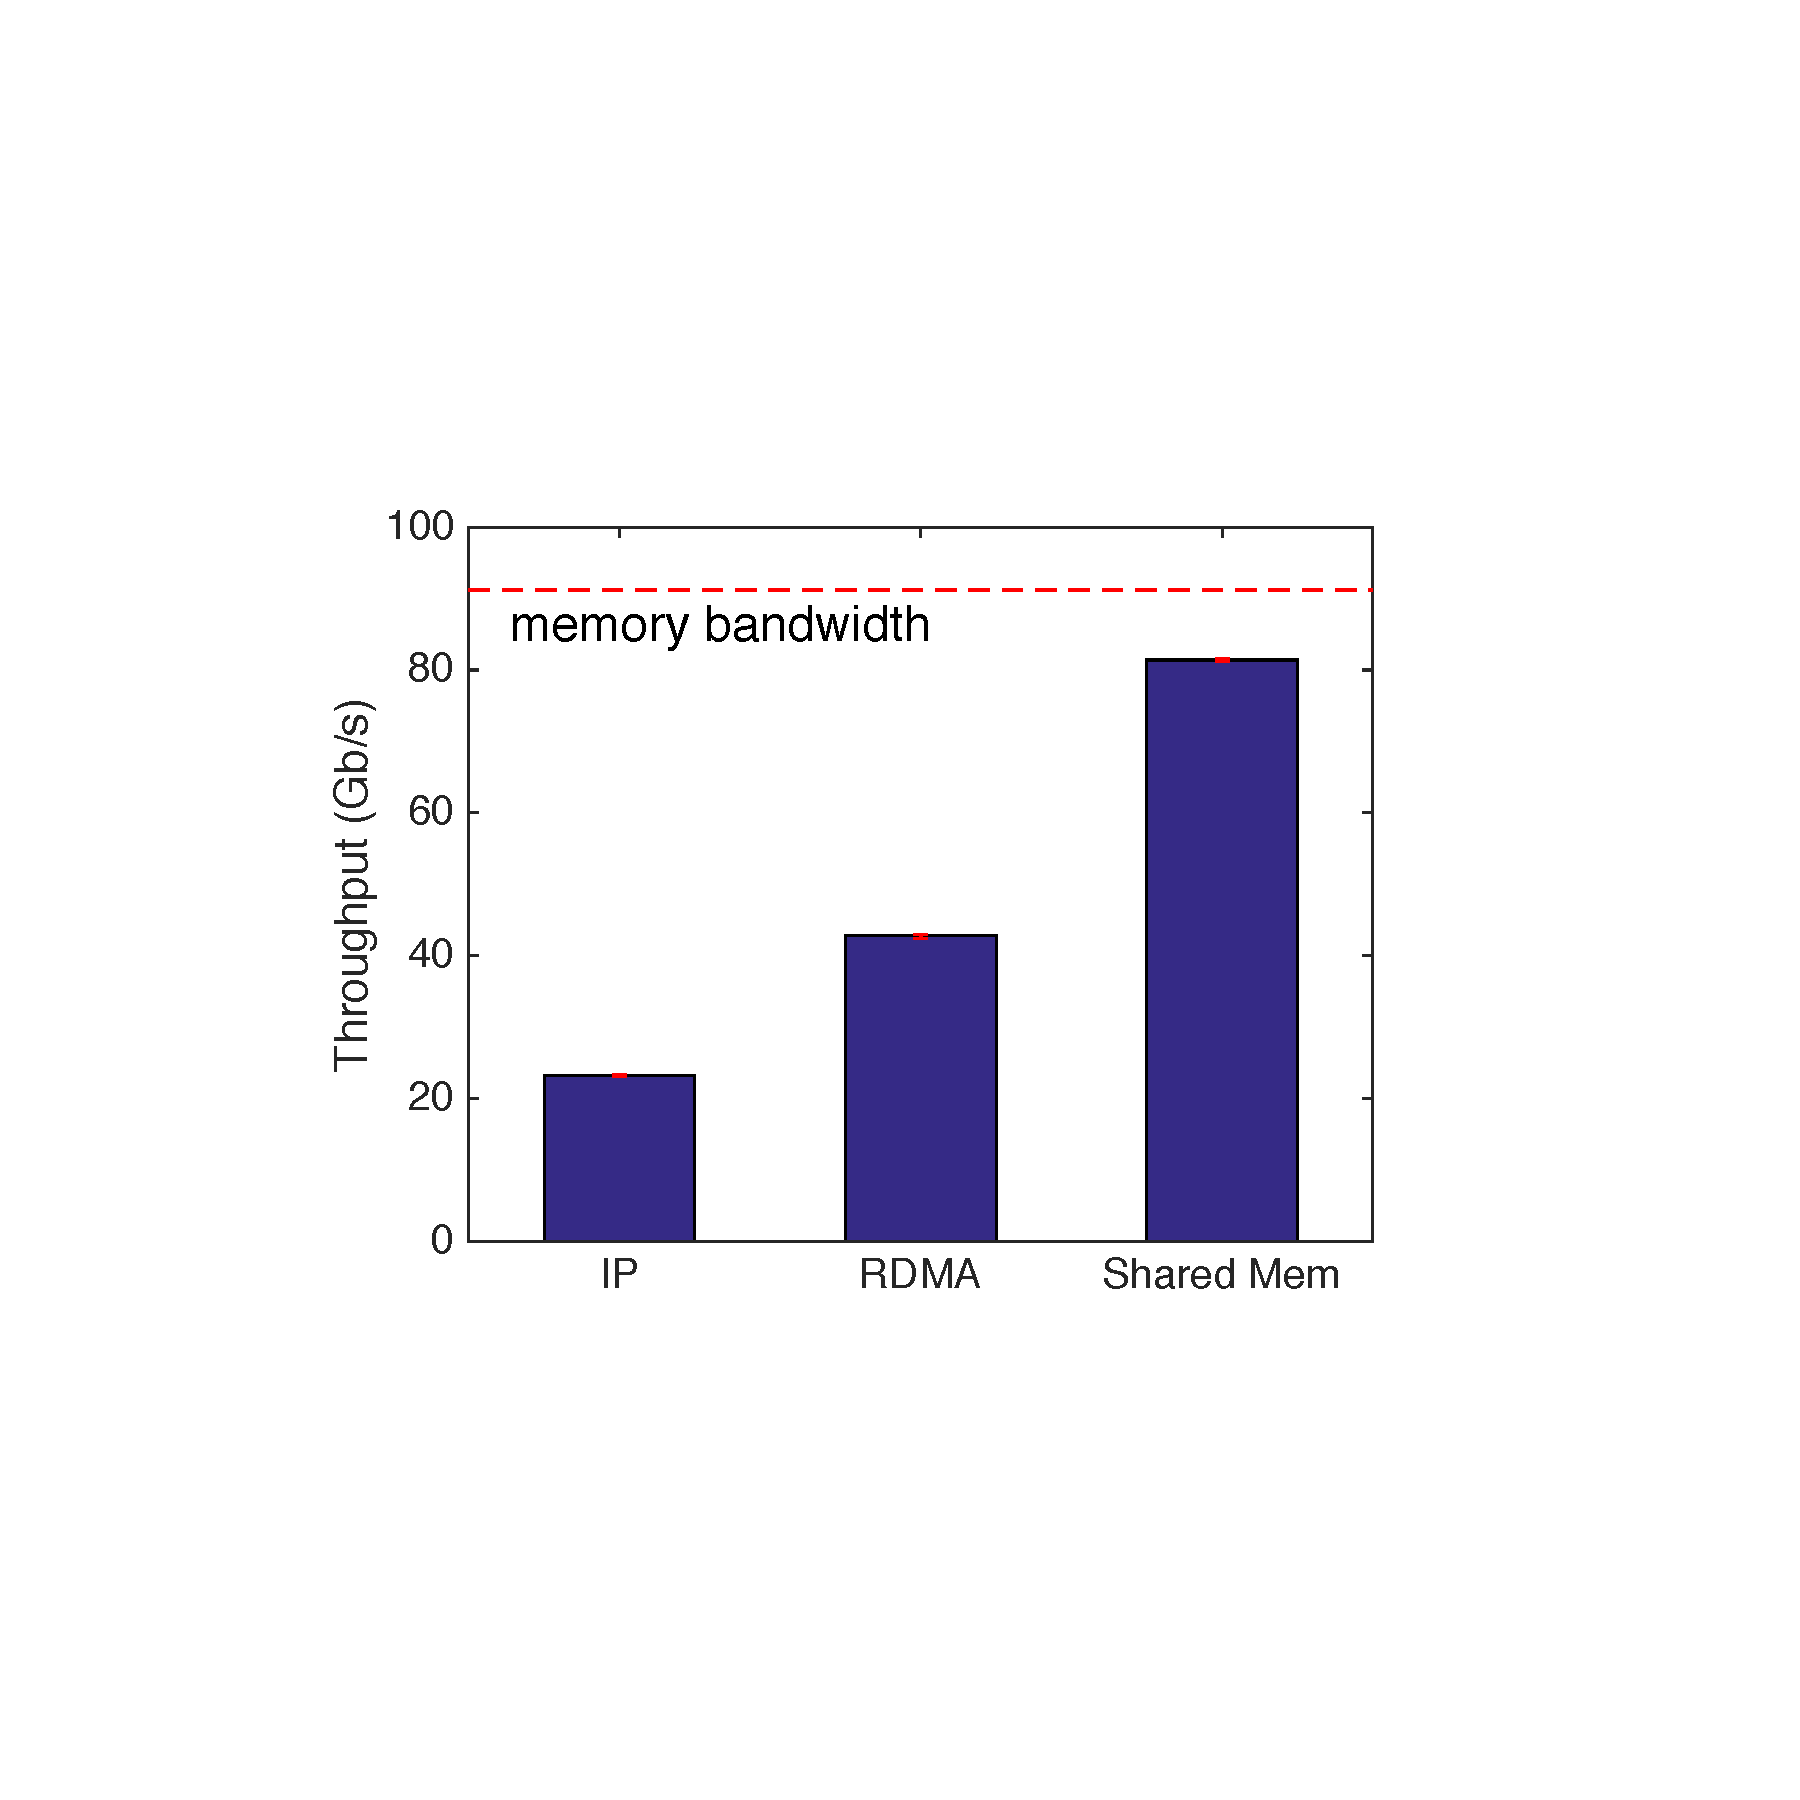
\includegraphics[width=0.32\textwidth]{figures/motivation/eval_baremetal_thr.pdf}      
     %\label{fig:eval_baremetal_thr}
     %\caption{} 
     \end{subfigure}      
     \begin{subfigure}[t]
     \centering 
     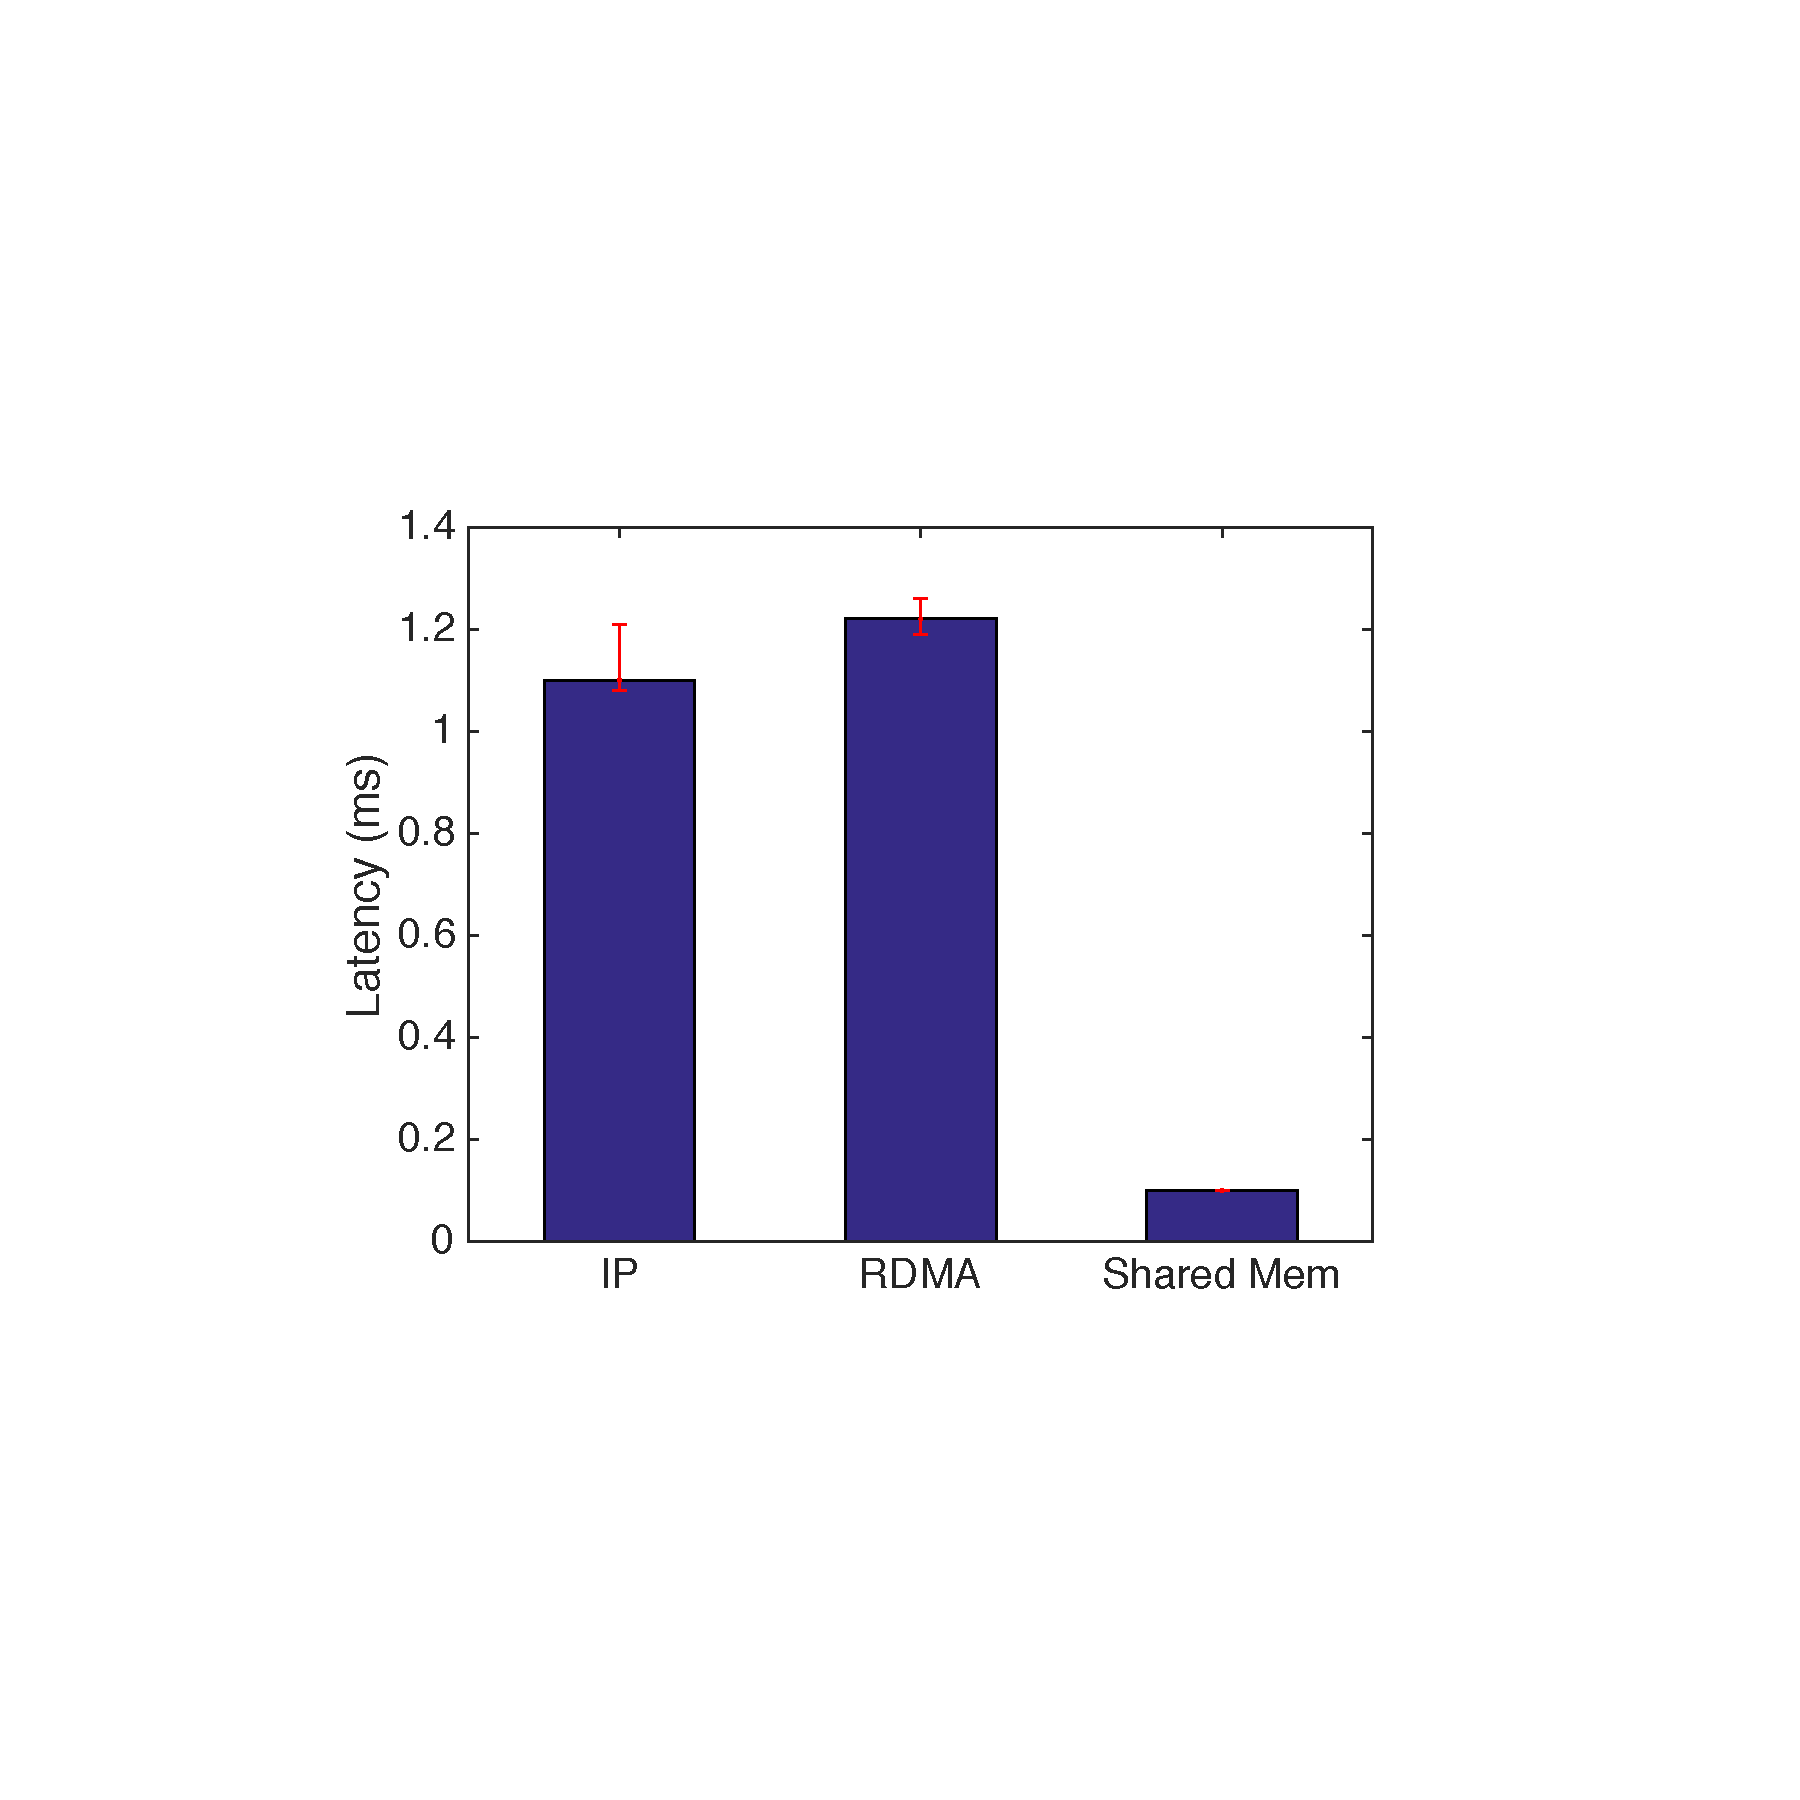
\includegraphics[width=0.32\textwidth]{figures/motivation/eval_baremetal_latency.pdf}      
     %\label{fig:eval_baremetal_latency}
     %\caption{} 
     \end{subfigure}      
     \begin{subfigure}[t]
     \centering 
     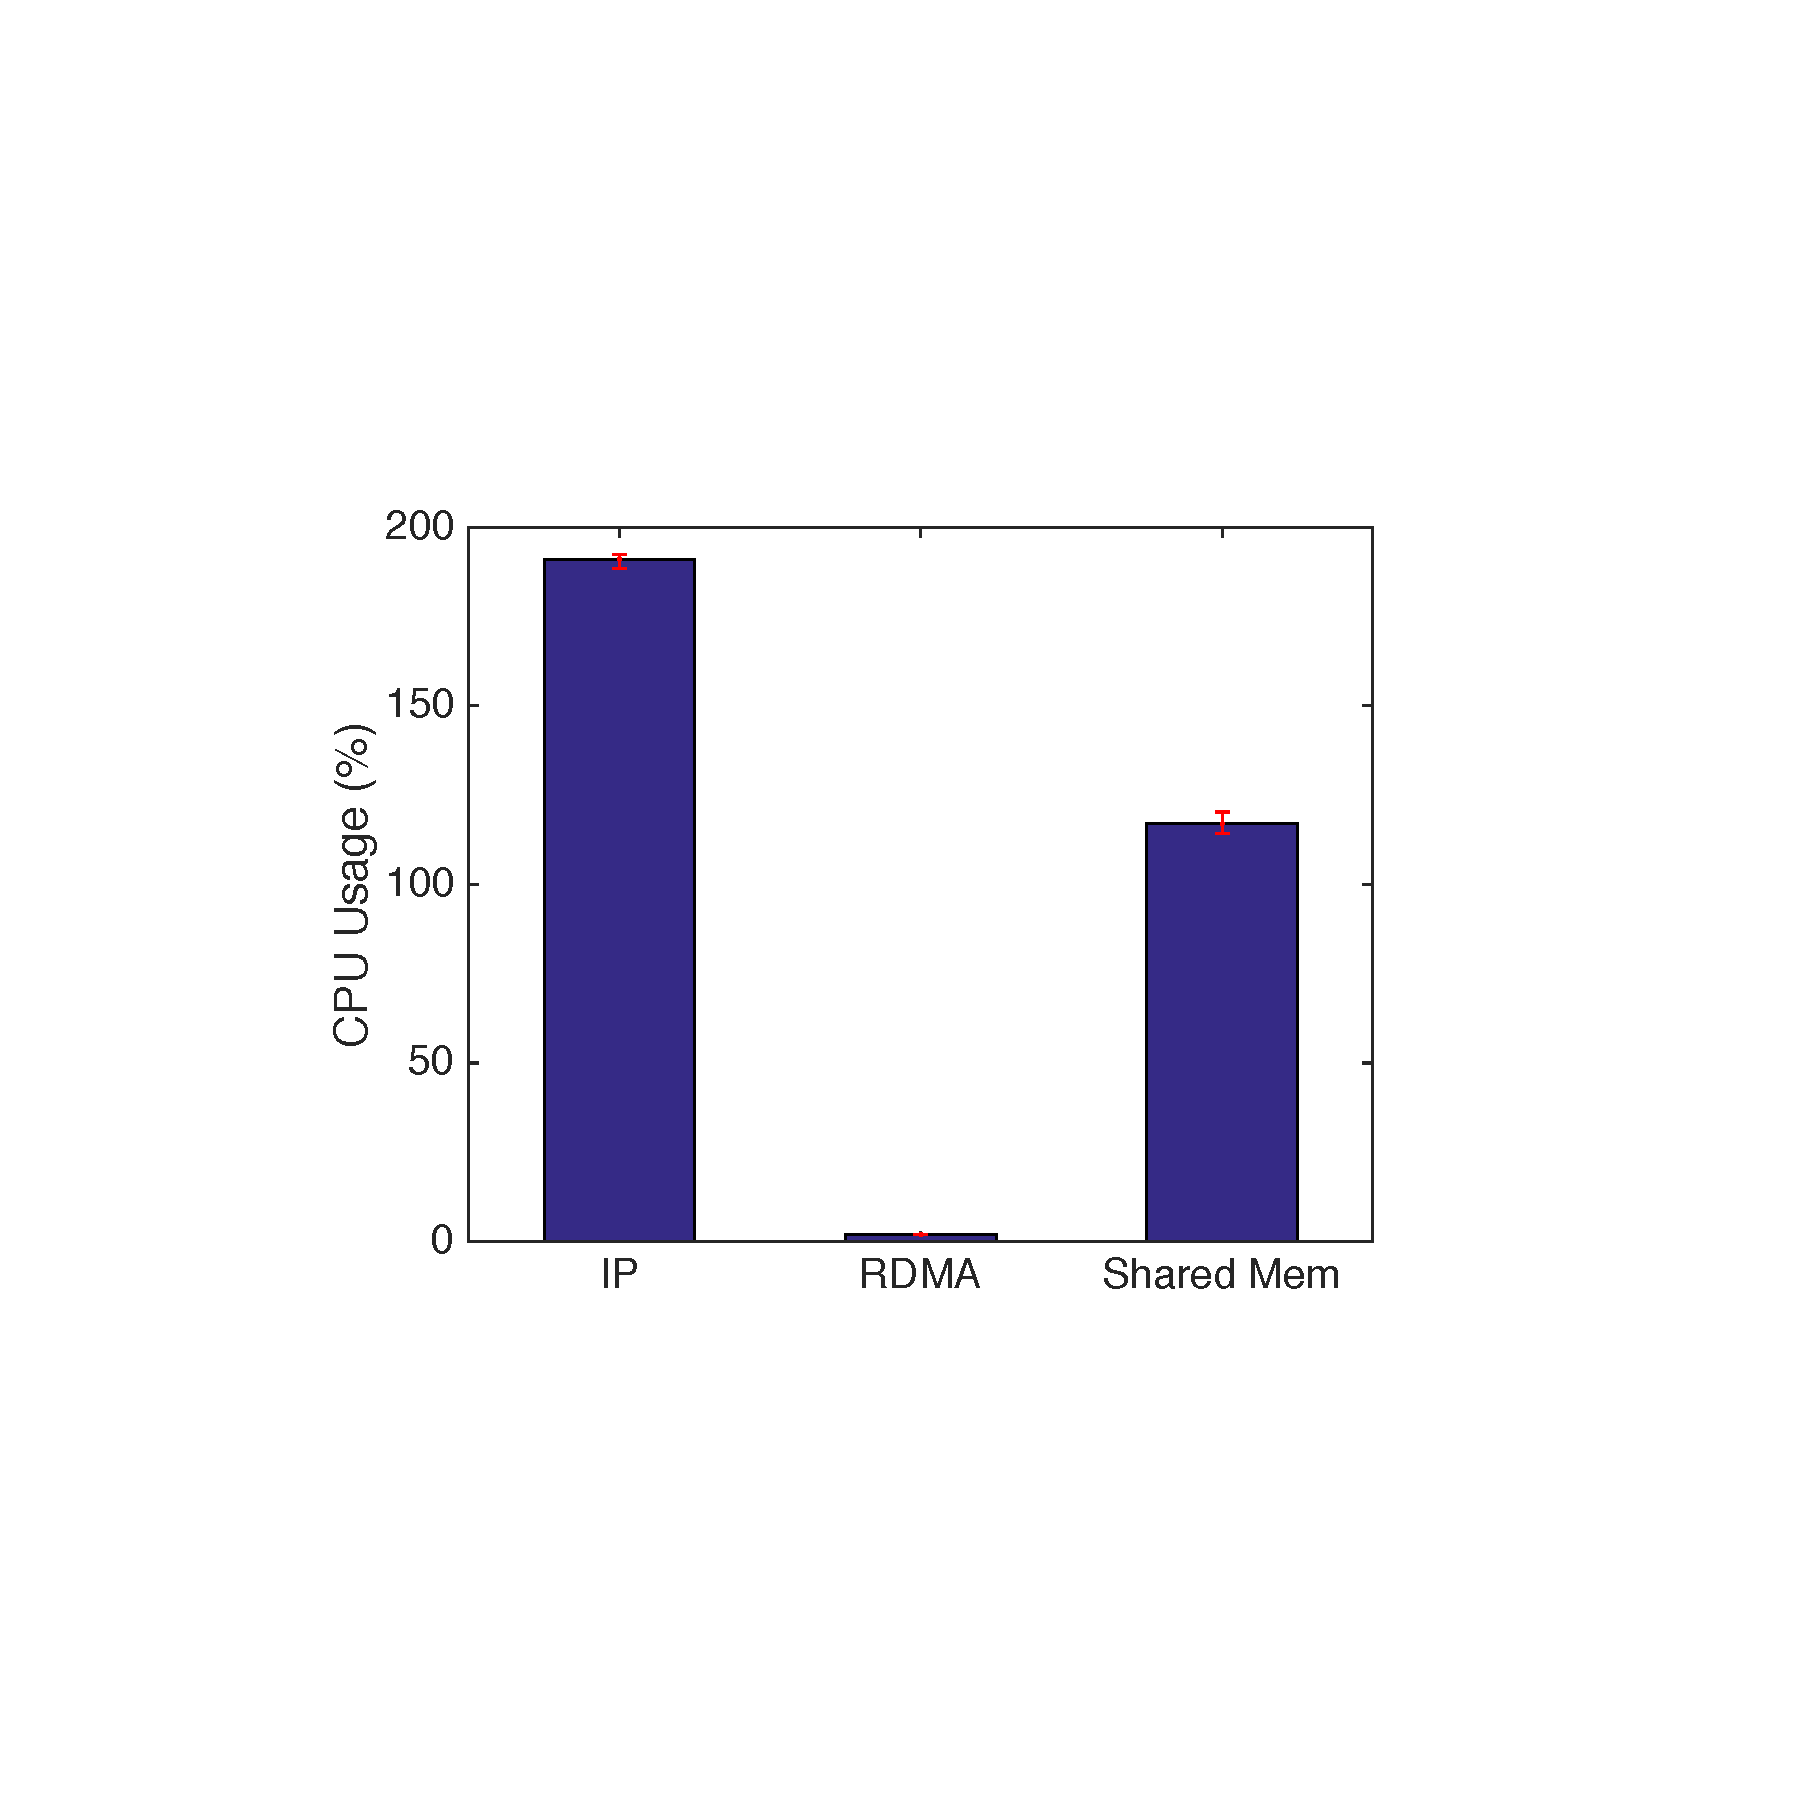
\includegraphics[width=0.32\textwidth]{figures/motivation/eval_baremetal_cpu.pdf}      
     %\label{fig:eval_baremetal_cpu}
     %\caption{} 
     \end{subfigure}           
     \label{fig:eval_baremetal_thr_latency_cpu}
     \caption{} 
\end{figure*} 

\begin{itemize}
  \item Communication via IP stack only achieves 27Gb/s throughput, 1 ms latency but uses near to 200\% of cpu.
  \item RDMA only improves the throughput to 40Gb/s for containers on the same machine, the latency is still 1ms, though it has a low cpu usage.
  \item Shared memory can achieve near-to-memory-bandwidth throughput, lowest latency, but still burns some cpu. 
\end{itemize}


\subsubsection{Host-mode vs. bridge mode}

\begin{figure}[!ht]
     \centering 
     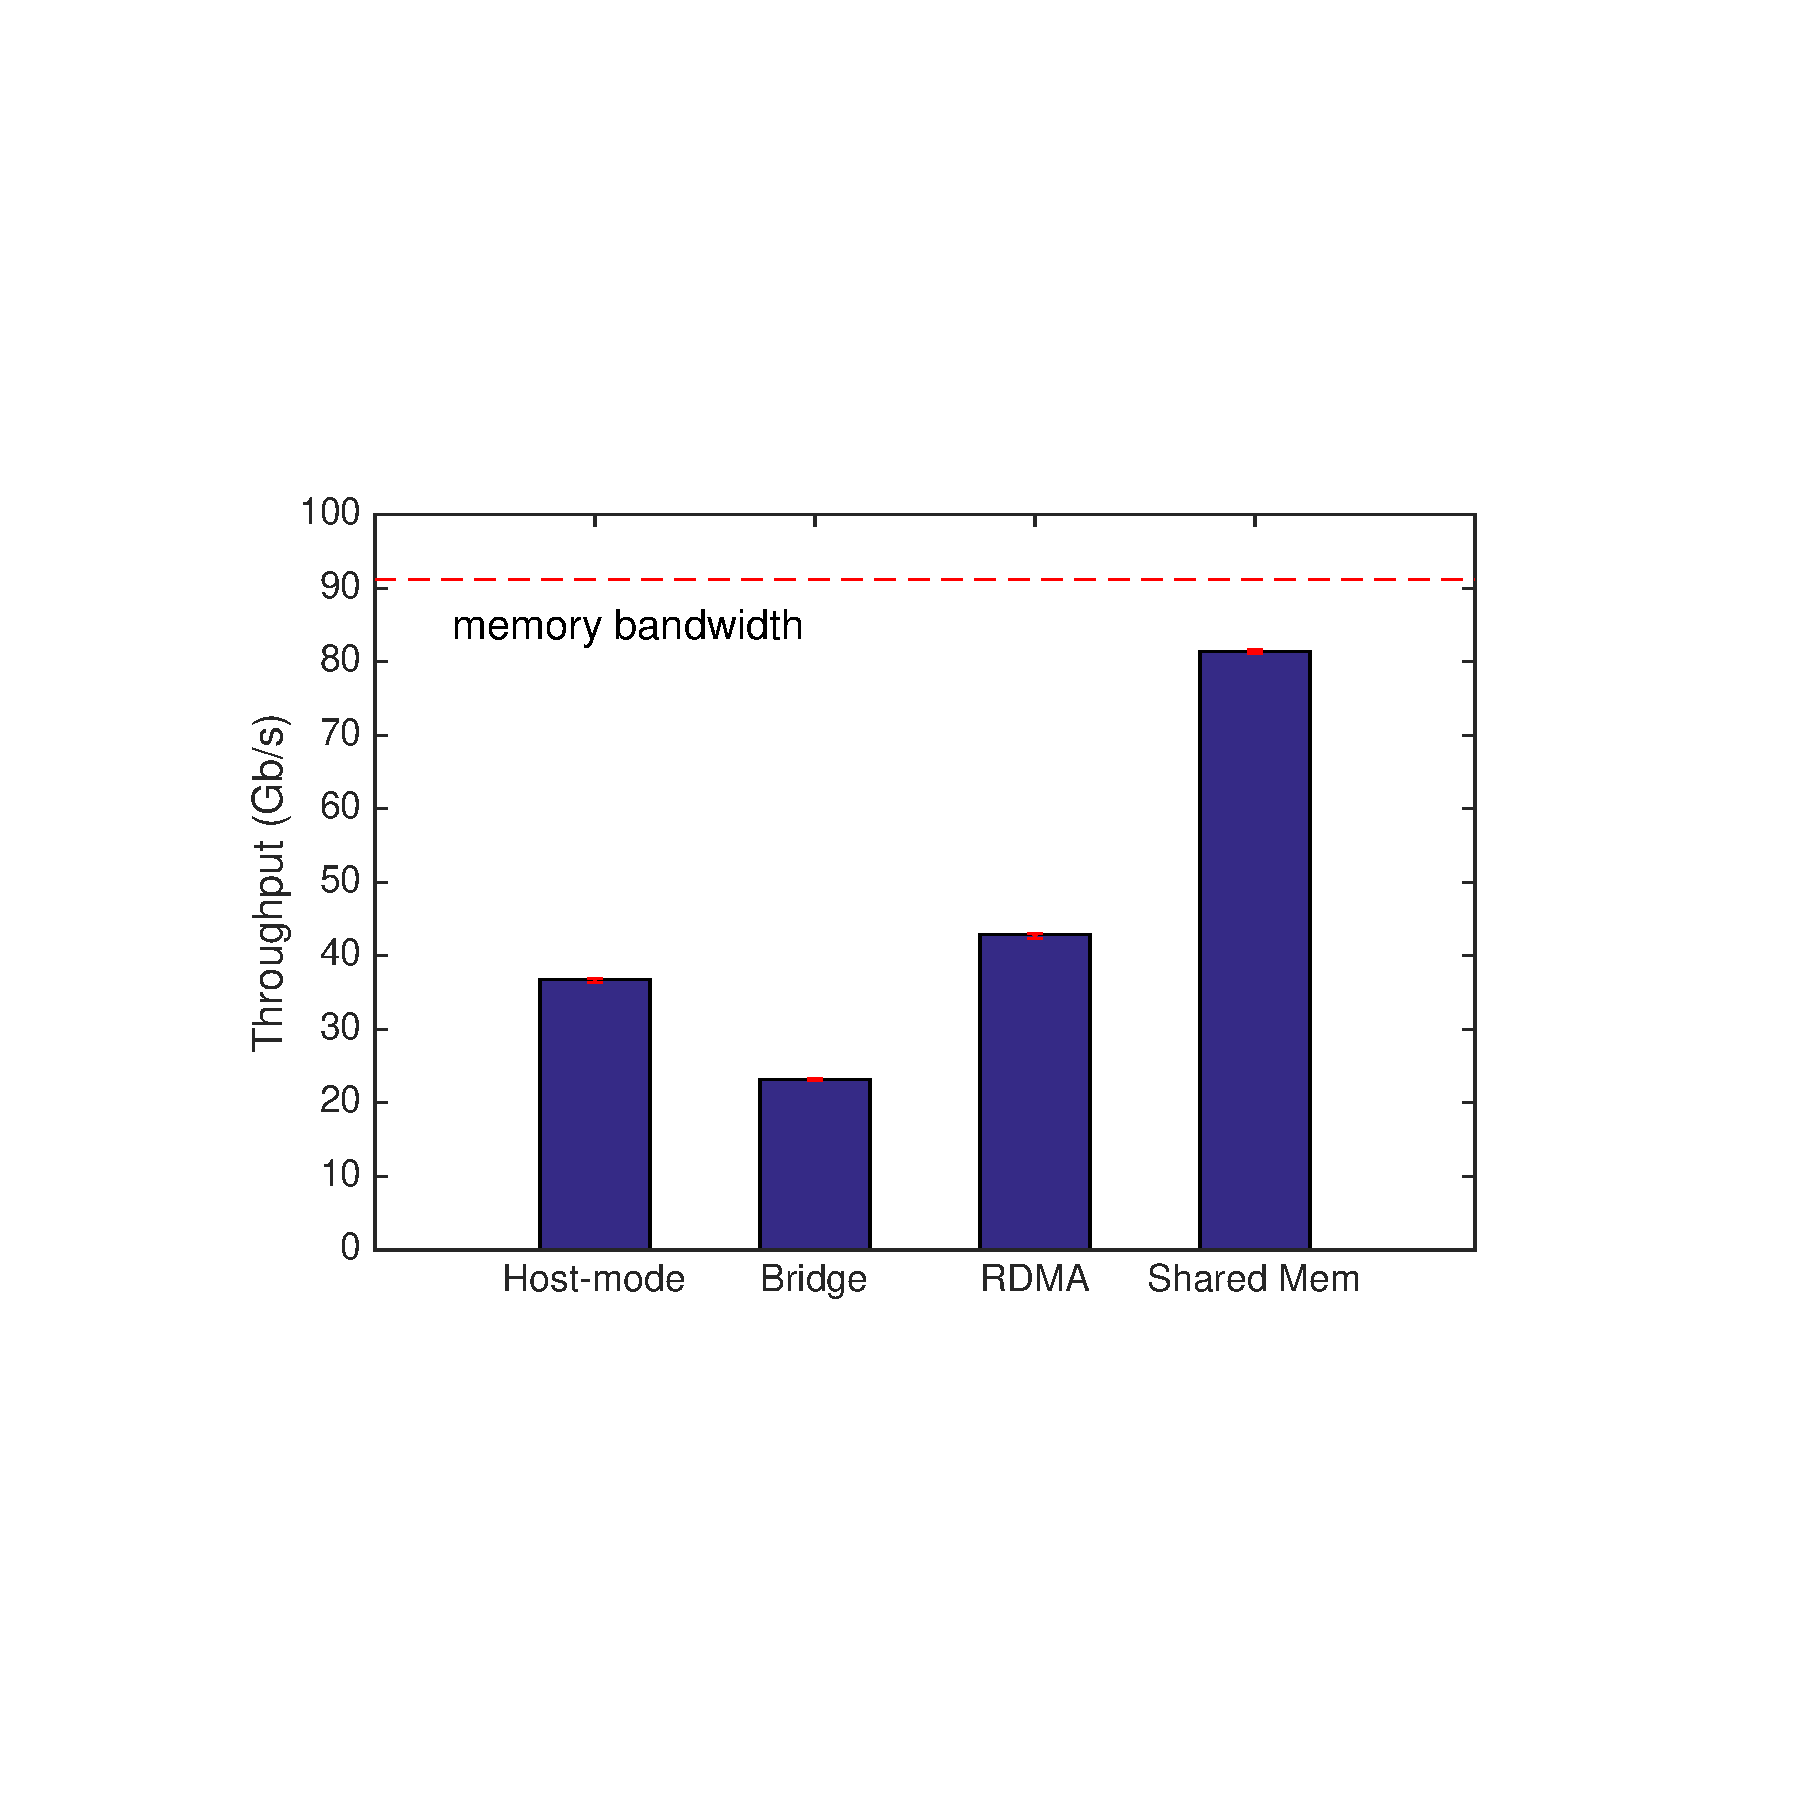
\includegraphics[width=3.35in]{figures/motivation/eval_bw_host_bridge.pdf} 
     \label{fig:eval_bw_host_bridge}
     \caption{ Host-mode vs. bridge mode vs. RDMA vs. shared memory.} 
\end{figure} 

\begin{itemize}
  \item Host-mode provides a better performance of 38 Gb/s. 
\end{itemize}

\subsection{Intra-host Network Performance}

\para{Throughput}

Three points: (1) TCP throughput is limited; (2) the bottleneck is CPU rather than memory bus for TCP/IP; (3) the bottleneck is NIC CPU for RDMA. (4) For intra-host cases, shared memory has the best performance.

Figure 1: throughput of single src-dst pair. Bar figure: x-axis: TCP/IP, RDMA and shared memory; y-axis: throughput;

Figure 2(a): throughput of multiple src-dst pair. Line figure: x-axis: number of pairs,; y-axis: throughput; Four lines: TCP/IP, RDMA, shared memory and memory bus.

Figure 2(b): CPU utilization. Line figure: x-axis: number of pairs,; y-axis: CPU utilization; Three lines: TCP/IP, RDMA, shared memory.

Figure 2(c): NIC CPU utilization. Line figure: x-axis: number of pairs,; y-axis: NIC CPU utilization; Three lines: TCP/IP, RDMA, shared memory.

\begin{figure}[!ht]
     \centering 
     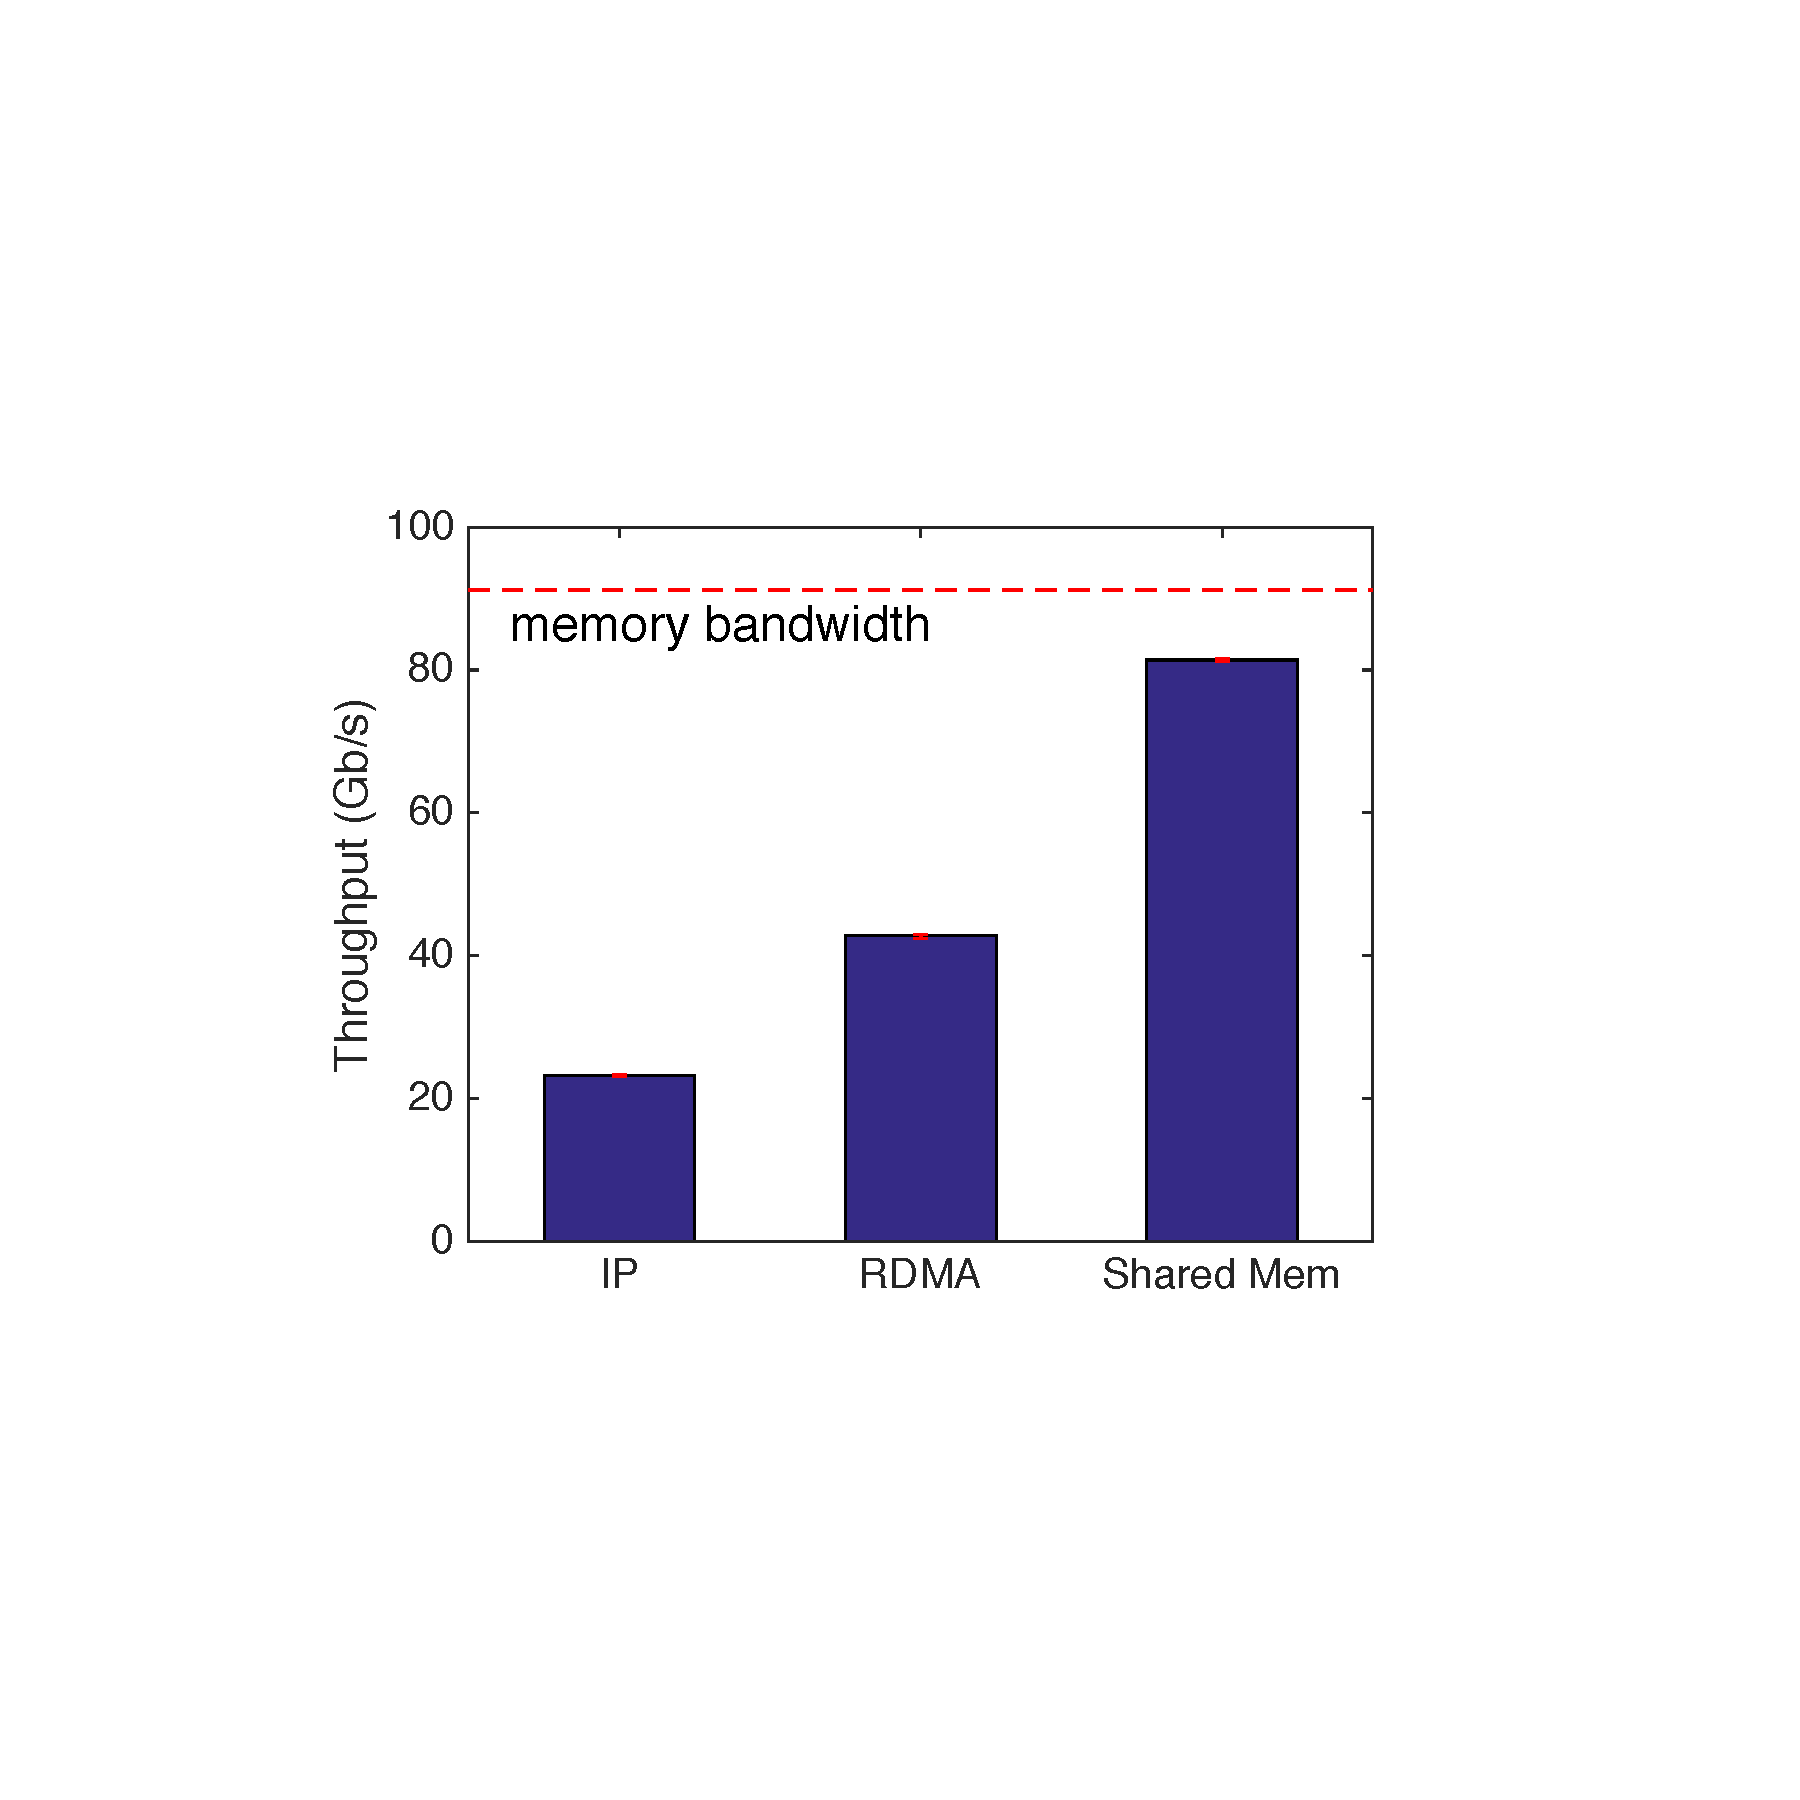
\includegraphics[width=3.35in]{figures/motivation/eval_baremetal_thr.pdf} 
     \caption{\label{fig:eval_baremetal_thr} The throughput of a pair of containers on the same bare metal communicating via IP stack, RDMA and shared memory. Communication via shared memory is close to the memory bandwidth.} 
\end{figure} 

\para{Latency}
Two points: (1) going through OS stack is increasing network latency; (2) The bottleneck is on system calls.

Figure 3: The stacked bar chart showing the total latency of TCP/IP, RDMA, shared memory and their components.

\begin{figure}[!ht]
     \centering 
     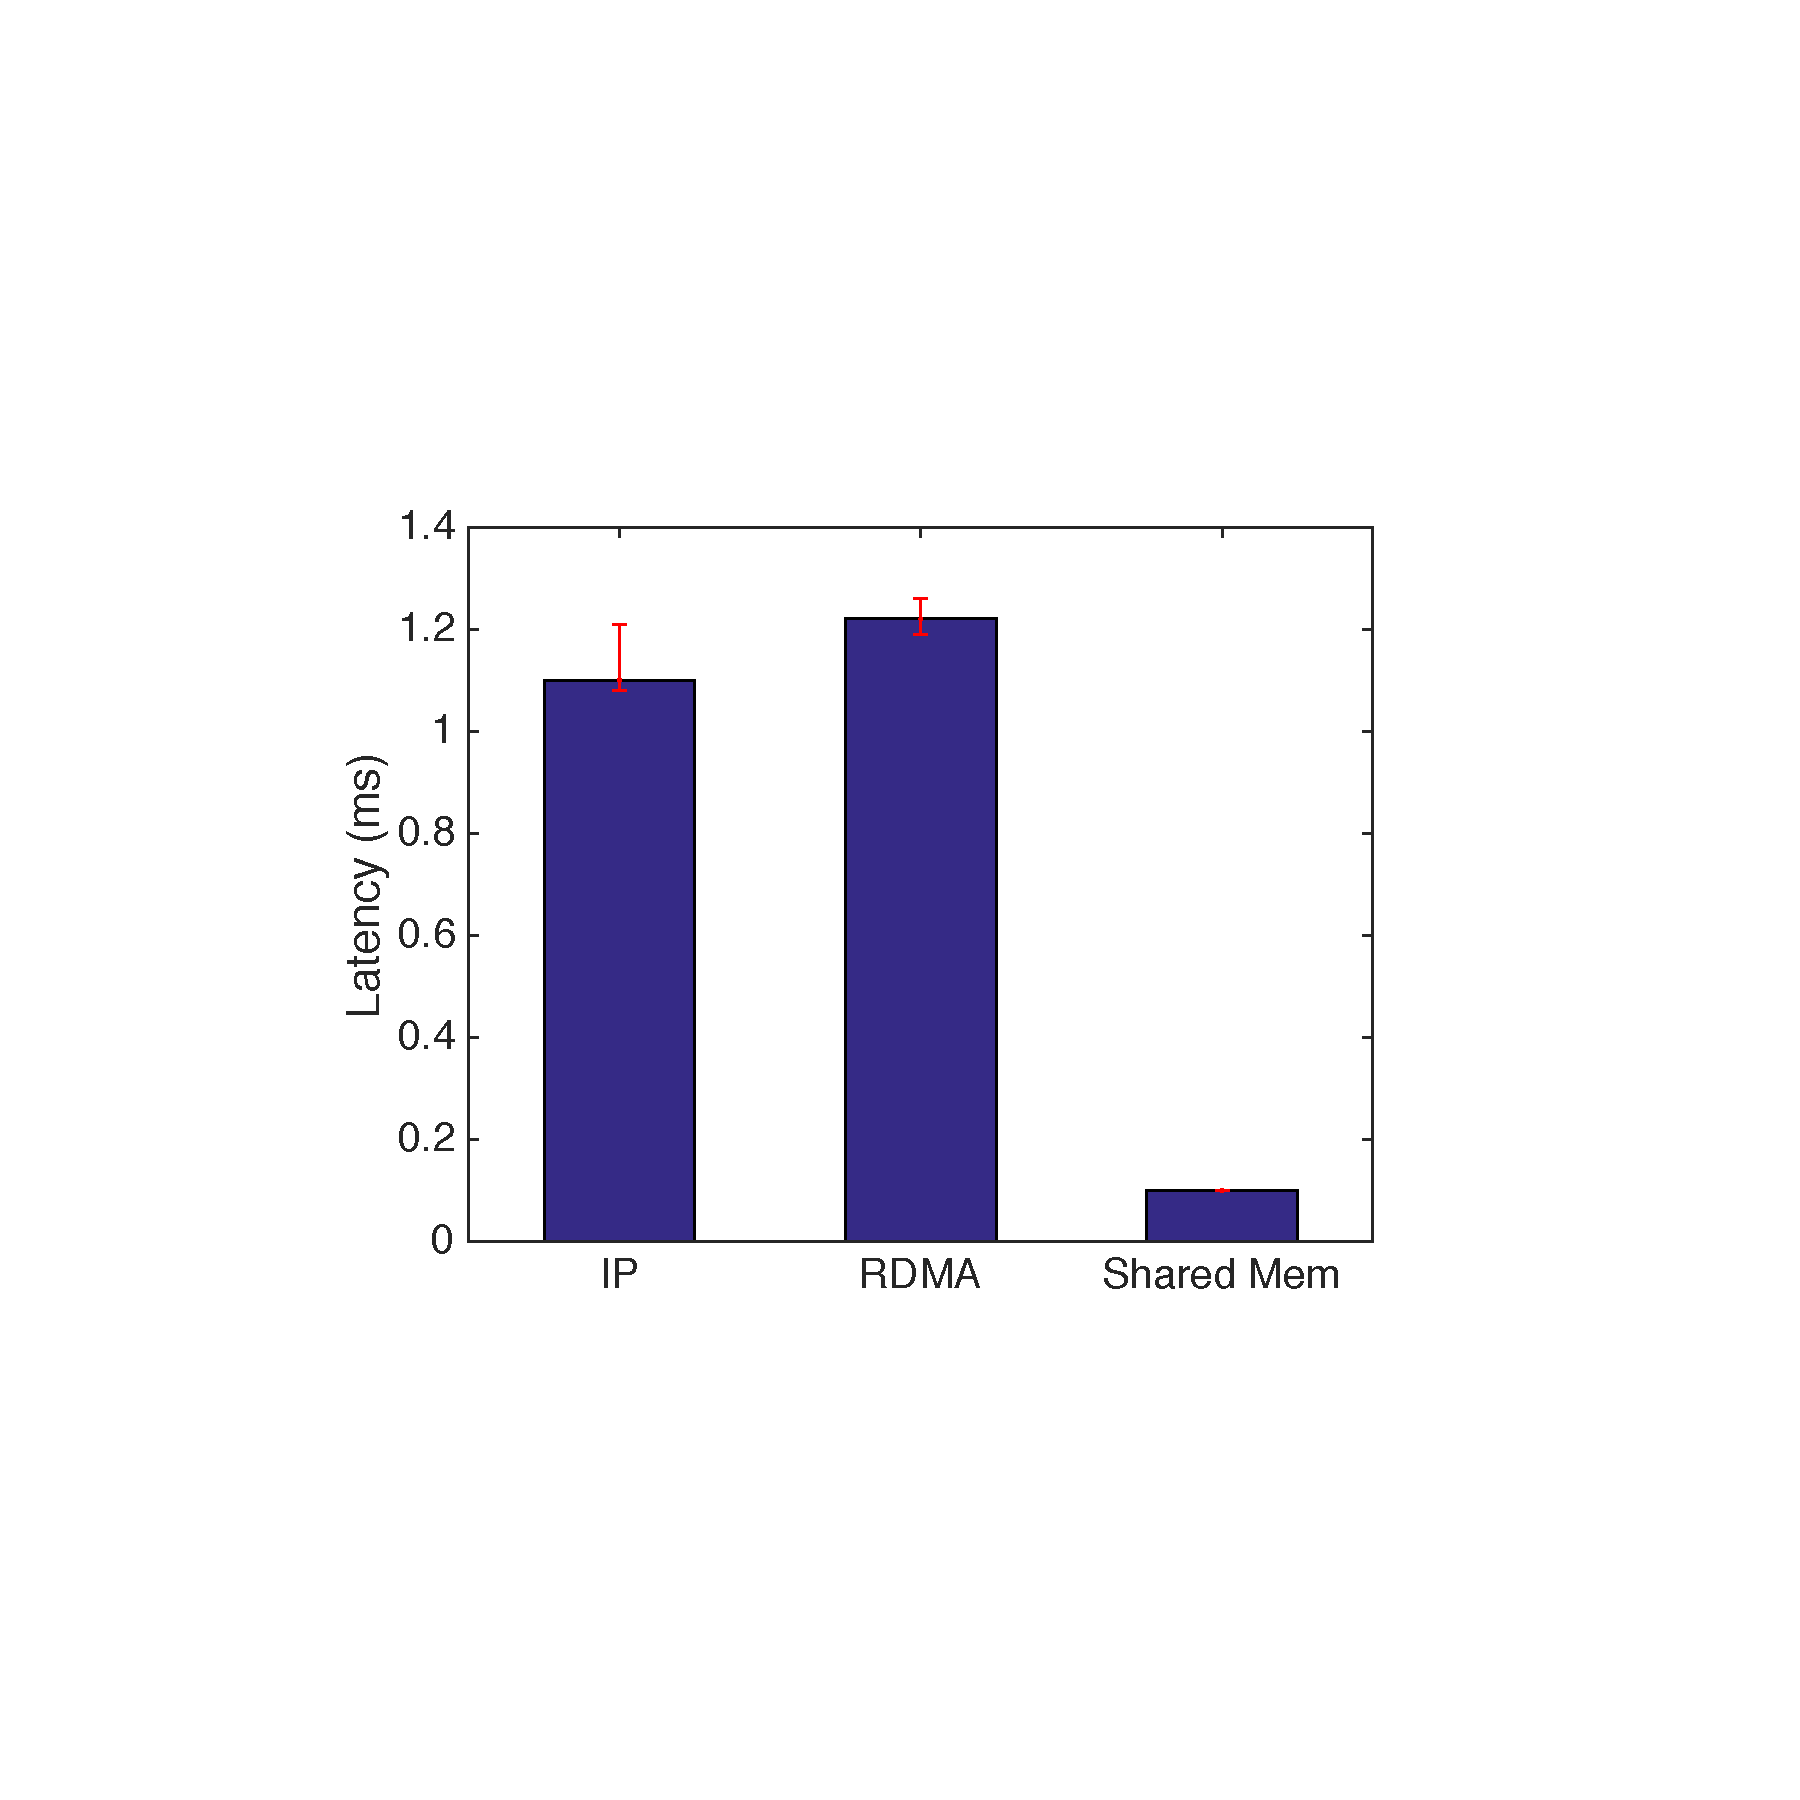
\includegraphics[width=3.35in]{figures/motivation/eval_baremetal_latency.pdf} 
     \caption{\label{fig:eval_baremetal_latency} The latency of a pair of containers on the same bare metal communicating via IP stack, RDMA and shared memory. Shared memory achieves the lowest latency.} 
\end{figure} 

\para{CPU Usage}

\begin{figure}[!ht]
     \centering 
     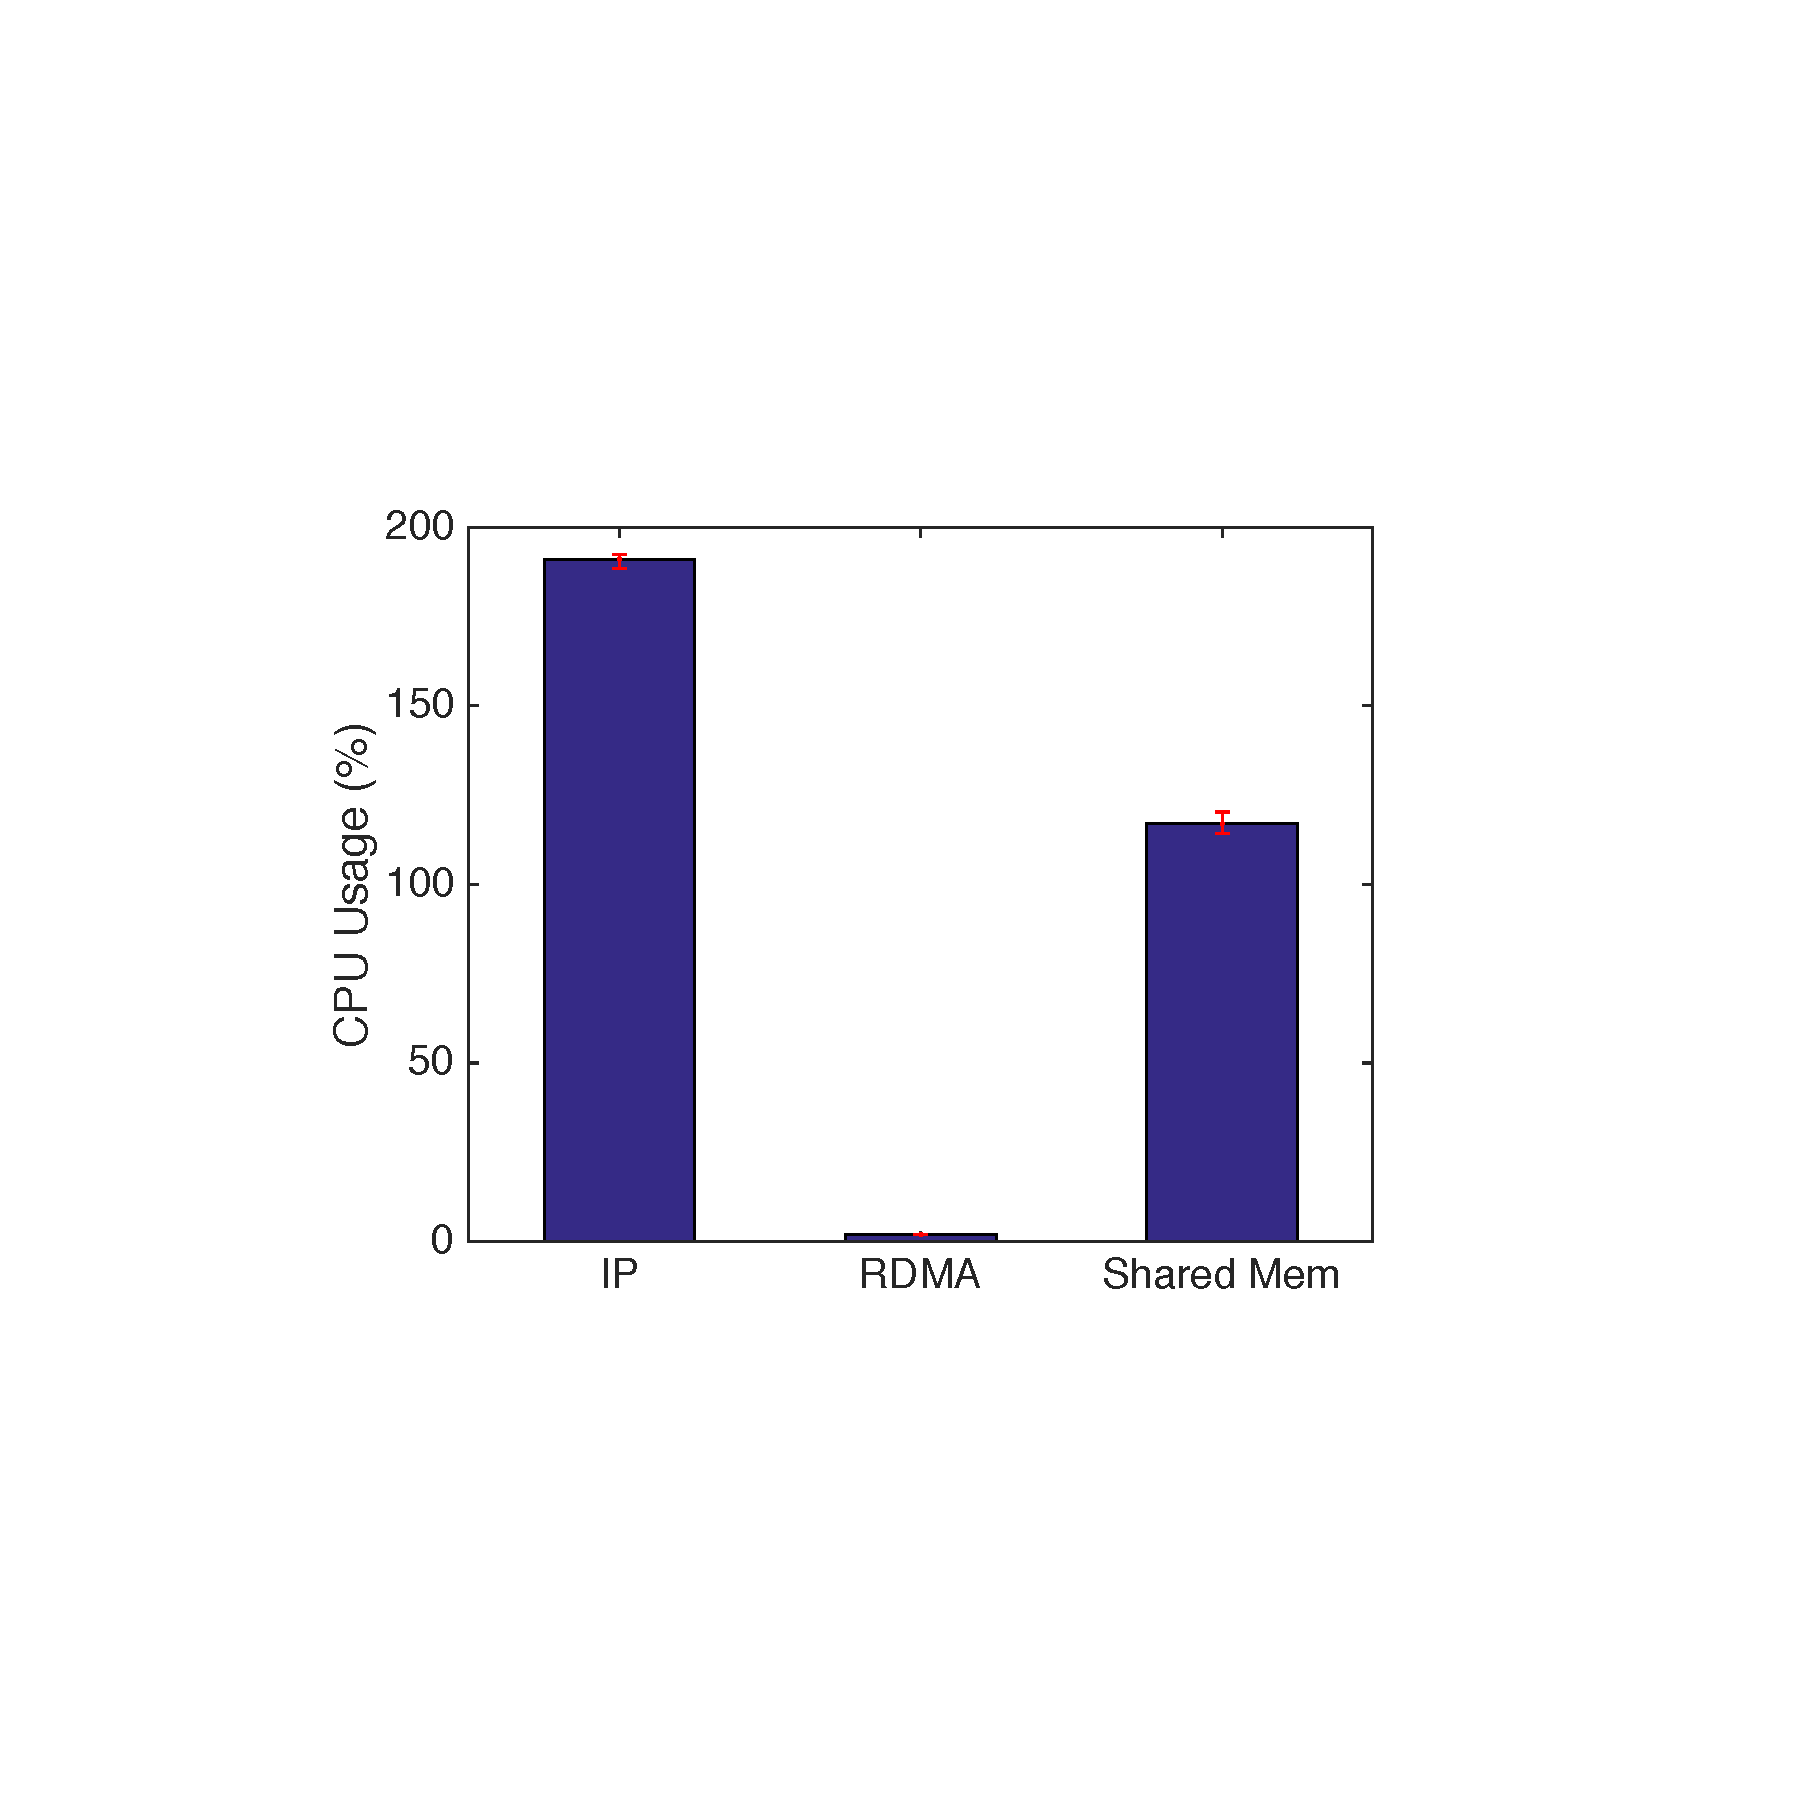
\includegraphics[width=3.35in]{figures/motivation/eval_baremetal_cpu.pdf} 
     \caption{\label{fig:eval_baremetal_cpu} The cpu usage of a pair of containers on the same bare metal communicating via IP stack, RDMA and shared memory. Communication via IP stack almost saturates 2 cpu cores.} 
\end{figure} 

% comment 
\fi
